% +--------------------------------------------------------------------+
% | Brian Cain 2014                                                    |
% | Kansas State University                                            |
% | Computer Information Science                                       |
% | Masters Report                                                     |
% +--------------------------------------------------------------------+

% +--------------------------------------------------------------------+
% | LaTeX Template                                                     |
% | for K-State Electronic Theses, Dissertations, and Reports          |
% |                                                                    |
% | Comments and guidelines for using the template are shown           |
% | within boxes like this one.                                        |
% |                                                                    |
% | Revised 6/30/06                                                    |
% | 9/14/06: Removed typos                                             |
% | 3/29/13: Commented out hypernat package                            |
% | 4/5/13: Changed to plain bib style
% | 5/17/13: added /cleardoublepage and /phantomsection to
% |          /bibliography to correct TOC page problem
% | 5/17/13: Fixed TOC problem with Dedication, Preface, etc.          |
% +--------------------------------------------------------------------+

% +--------------------------------------------------------------------+
% | Your paper should contain the following sections, except where     |
% | indicated as optional, in the order shown.  Also, all headings     |
% | shown with an asterisk (*) must be centered and in uppercase       |
% | letters:                                                           |
% |                                                                    |
% | Abstract Title Page (doctoral dissertations only)                  |
% | ABSTRACT* (doctoral dissertations only)                            |
% | Title Page                                                         |
% | Copyright Page (Optional - only needed if copyrighting)            |
% | ABSTRACT *                                                         |
% | TABLE OF CONTENTS *                                                |
% | LIST OF FIGURES *                                                  |
% | LIST OF TABLES*                                                    |
% | ACKNOWLEDGMENTS* (Optional)                                        |
% | DEDICATION * (Optional)                                            |
% | PREFACE * (Optional)                                               |
% | Individual Chapters                                                |
% | References and/or bibliography                                     |
% | Appendices (as needed)                                             |
% +--------------------------------------------------------------------+

% +--------------------------------------------------------------------+
% | The LaTex keyword \documentclass selects a particular class to     |
% | associate with the document.  The current documentclass            |
% | {class_diss} generates a Table of Contents that has leading dots   |
% | only on chapter subheadings.  If you prefer a Table of Contents    |
% | that has leading dots for all entries, replace {class_diss}        |
% | with {Mydiss} in the command below.                                |
% |                                                                    |
% +--------------------------------------------------------------------+

\documentclass[final, 12pt,oneside]{class_diss}

% +--------------------------------------------------------------------+
% | The bibliography style is set to a generic superscript. Other      |
% | styles are available in the styles directory.  To use an           |
% | author/year style, you'll need to make several adjustments:        |
% |   1.  In the \bibliographystyle command below, replace "unsrtnat"  |
% |       with the desired style from the \styles directory, e.g.,     |
% |       \bibliographystyle{styles\apa}                               |
% |   2.  In the \bibpunct command (several lines below), change the   |
% |       "s" to an "a"                                                |
% |   3.  Use "\citep" rather than "\cite" when making a citation in   |
% |       the text.                                                    |
% +--------------------------------------------------------------------+

\bibliographystyle{unsrtnat}

% +--------------------------------------------------------------------+
% | Now, we add in all external packages that we will use throughout   |
% | the document.  You can add other packages as needed.
% +--------------------------------------------------------------------+

%\usepackage{     caption2} % Customize captions a bit more
\usepackage{      amsmath} % American Mathematics Society standards
%\usepackage{      wrapfig} % Wraps text around a figure or table
\usepackage{     graphicx} % Extended graphics package.
%\usepackage{     fancyhdr} % Efficiently handles headers and footers
%\usepackage{       braket} % Bra-Ket notation package
%\usepackage{     mathrsfs} % Specialized Math fonts (Hamiltonian, etc.)
%\usepackage{boxedminipage} % Boxed text can be produced
%\usepackage{     setspace} % Controls line spacing via \begin{space}

\usepackage{amsxtra}
\usepackage{amssymb}
\usepackage{amsthm}
\usepackage{latexsym}
\usepackage{setspace}

% +--------------------------------------------------------------------+
% | The color package allows one to select colors for hyperlinking     |
% | (see below).                                                       |
% +--------------------------------------------------------------------+

\usepackage[usenames]{color}


% +--------------------------------------------------------------------+
% | New package for code syntax highlighting                           |
% +--------------------------------------------------------------------+

\usepackage{minted}

% +--------------------------------------------------------------------+
% | Colors defined for use with this template.                         |
% +--------------------------------------------------------------------+

\definecolor{  Pink}{rgb}{1.0, 0.5, 0.5}
\definecolor{Maroon}{rgb}{0.8, 0.0, 0.0}

% +--------------------------------------------------------------------+
% | In the commands below, we use the 'natbib' package, and specify    |
% | the 'sort&compress' option, which condenses                        |
% | citations from (1,2,3,5,9,10,11) to (1-3,5,9-11).  The 'bibpunct'  |
% | option selects various parameters for how the citation will be     |
% | displayed.  In this case, only the comma (separation between       |
% | citations) and the 's' (superscript) arguments are chosen.  The    |
% | other curly braces deal with how to 'wrap' the citation (using     |
% | parentheses, brackets, etc.) and are not needed for the chosen     |
% | style.                                                             |
% +--------------------------------------------------------------------+

\usepackage{natbib}
\bibpunct{}{}{,}{s}{}{}
%\usepackage{hypernat}

% +--------------------------------------------------------------------+
% | Lastly, the hyperref package allows one to hyperlink cross-        |
% | references and figures in a LaTeX document.                        |
% | 3/29/13 - Hypernat package commented out because  it is no longer      |
% | needed with later versions of hyperref and natbib.                 |
% +--------------------------------------------------------------------+

\usepackage[pdftex, plainpages=false, pdfpagelabels]{hyperref}

\hypersetup{
    linktocpage=true,
    colorlinks=true,
    bookmarks=true,
    citecolor=blue,
    urlcolor=red,
    linkcolor=Maroon,
    citebordercolor={1 0 0},
    urlbordercolor={1 0 0},
    linkbordercolor={.7 .8 .8},
    breaklinks=true,
    pdfpagelabels=true,
    }

% +--------------------------------------------------------------------+
% | Page margins are set on 1 inch on all sides.                       |
% +--------------------------------------------------------------------+

\topmargin      = -0.56in
\textheight     =  8.60in
\textwidth      =  6.46in
\oddsidemargin  =  0.02in


% +--------------------------------------------------------------------+
% | The document finally begins here.                                  |
% +--------------------------------------------------------------------+

\doublespacing
\begin{document}

% +--------------------------------------------------------------------+
% | Define macro here.                                                 |
% +--------------------------------------------------------------------+

\newcommand{\projectName}{ANCOR Dashboard}
\newcommand{\ancor}{ANCOR}
\newcommand{\ancorcli}{ANCOR-CLI}

% +--------------------------------------------------------------------+
% | Masters Students -- You Need to Make Some Changes Here

% | The Abstract Title page and Abstract following the Abstract Title
% | page are required only for doctoral dissertations.  For masters
% | theses or reports, comment out or delete the following 7 lines:
% | % +--------------------------------------------------------------------+
% | Abstract Title Page
% |
% |This page is required only for doctoral dissertations.
% +--------------------------------------------------------------------+

% +--------------------------------------------------------------------+
% | This page should not contain a page number.  We use the
% | \thispagestyle[empty] command below to suppress page numbers
% | and other style elements.
% +--------------------------------------------------------------------+

\thispagestyle{empty}

% +--------------------------------------------------------------------+
% | The Abstract Title page begins here                                |
% +--------------------------------------------------------------------+

\pdfbookmark[0]{Title Page}{PDFTitlePage}
%\setcounter{page}{1}

\begin{center}

   \vspace{1cm}

% +--------------------------------------------------------------------+
% | Enter the title of your ETDR below.  Use ALL CAPITAL LETTERS.
% +--------------------------------------------------------------------+

   \large MY MASTERS REPORT TITLE\\

   \vspace{0.5cm}

   by\\

   \vspace{0.5cm}

% +--------------------------------------------------------------------+
% | Enter your name below in ALL CAPITAL LETTERS.
% +--------------------------------------------------------------------+

   \large BRIAN CAIN\\

   \vspace{0.5cm}

% +--------------------------------------------------------------------+
% | List previous degrees in mixed case. Include the abbreviation for  |
% | the degree, the name of the university, and the year separated by  |
% | commas. For example:                                               |
% |                                                                    |
% |    B.A., University of Illinois, 2000                              |
% |                                                                    |
% | If desired, it is acceptable to include a city or country with     |
% | the university name. For example:                                  |
% |                                                                    |
% |    B.S., Jillian University, China, 2002                           |
% +--------------------------------------------------------------------+

   B.S., Kansas State University, Manhattan KS, 2012\\

   \vspace{0.55cm}
   \rule{2in}{0.5pt}\\
   \vspace{0.75cm}

   {\large AN ABSTRACT OF A DISSERTATION}\\

   \vspace{0.5cm}
   \begin{singlespace}
   submitted in partial fulfillment of the\\
   requirements for the degree\\
   \end{singlespace}

   \vspace{0.5cm}

% +--------------------------------------------------------------------+
% | On the line below, enter the name of your earned degree in ALL
% | CAPITAL LETTERS.  For example: DOCTOR OF PHILOSOPHY
% +--------------------------------------------------------------------+


   {\large MASTERS OF COMPUTER SCIENCE}\\
   \vspace{0.5cm}

% +--------------------------------------------------------------------+
% | On the two lines below, enter the name of your department and the
% | name of the college in mixed case.  For example:
% |
% |     Biochemistry Department
% |     College of Arts and Sciences
% +--------------------------------------------------------------------+

   \begin{singlespace}
   Computing and Information Sciences\\
   College of Engineering\\
   \end{singlespace}

   \vspace{0.5cm}

   \begin{singlespace}
   {\Large KANSAS STATE UNIVERSITY}\\
   Manhattan, Kansas\\
   \end{singlespace}

% +--------------------------------------------------------------------+
% | On the line below, enter the year of your graduation.  The year
% | should be the only text on the line.  For example:
% |
% |     2006
% +--------------------------------------------------------------------+

   2014\\
   \vspace{1cm}

\end{center}
 through \end{abstract}.  You will also
% | need to uncomment two lines under "Abstract" below.
% |
% +--------------------------------------------------------------------+

% % +--------------------------------------------------------------------+
% | Abstract Title Page
% |
% |This page is required only for doctoral dissertations.
% +--------------------------------------------------------------------+

% +--------------------------------------------------------------------+
% | This page should not contain a page number.  We use the
% | \thispagestyle[empty] command below to suppress page numbers
% | and other style elements.
% +--------------------------------------------------------------------+

\thispagestyle{empty}

% +--------------------------------------------------------------------+
% | The Abstract Title page begins here                                |
% +--------------------------------------------------------------------+

\pdfbookmark[0]{Title Page}{PDFTitlePage}
%\setcounter{page}{1}

\begin{center}

   \vspace{1cm}

% +--------------------------------------------------------------------+
% | Enter the title of your ETDR below.  Use ALL CAPITAL LETTERS.
% +--------------------------------------------------------------------+

   \large MY MASTERS REPORT TITLE\\

   \vspace{0.5cm}

   by\\

   \vspace{0.5cm}

% +--------------------------------------------------------------------+
% | Enter your name below in ALL CAPITAL LETTERS.
% +--------------------------------------------------------------------+

   \large BRIAN CAIN\\

   \vspace{0.5cm}

% +--------------------------------------------------------------------+
% | List previous degrees in mixed case. Include the abbreviation for  |
% | the degree, the name of the university, and the year separated by  |
% | commas. For example:                                               |
% |                                                                    |
% |    B.A., University of Illinois, 2000                              |
% |                                                                    |
% | If desired, it is acceptable to include a city or country with     |
% | the university name. For example:                                  |
% |                                                                    |
% |    B.S., Jillian University, China, 2002                           |
% +--------------------------------------------------------------------+

   B.S., Kansas State University, Manhattan KS, 2012\\

   \vspace{0.55cm}
   \rule{2in}{0.5pt}\\
   \vspace{0.75cm}

   {\large AN ABSTRACT OF A DISSERTATION}\\

   \vspace{0.5cm}
   \begin{singlespace}
   submitted in partial fulfillment of the\\
   requirements for the degree\\
   \end{singlespace}

   \vspace{0.5cm}

% +--------------------------------------------------------------------+
% | On the line below, enter the name of your earned degree in ALL
% | CAPITAL LETTERS.  For example: DOCTOR OF PHILOSOPHY
% +--------------------------------------------------------------------+


   {\large MASTERS OF COMPUTER SCIENCE}\\
   \vspace{0.5cm}

% +--------------------------------------------------------------------+
% | On the two lines below, enter the name of your department and the
% | name of the college in mixed case.  For example:
% |
% |     Biochemistry Department
% |     College of Arts and Sciences
% +--------------------------------------------------------------------+

   \begin{singlespace}
   Computing and Information Sciences\\
   College of Engineering\\
   \end{singlespace}

   \vspace{0.5cm}

   \begin{singlespace}
   {\Large KANSAS STATE UNIVERSITY}\\
   Manhattan, Kansas\\
   \end{singlespace}

% +--------------------------------------------------------------------+
% | On the line below, enter the year of your graduation.  The year
% | should be the only text on the line.  For example:
% |
% |     2006
% +--------------------------------------------------------------------+

   2014\\
   \vspace{1cm}

\end{center}

% 
% \begin{abstract}
%    \setcounter{page}{-1}
%    \pdfbookmark[0]{Abstract}{PDFAbstractPage}
%    % +--------------------------------------------------------------------+
% | Abstract Page
% +--------------------------------------------------------------------+

\pagestyle{empty}
%\vspace{1cm}
\setlength{\baselineskip}{0.8cm}

%\indent

% +--------------------------------------------------------------------+
% | Enter the text of your abstract below, maximum of 350 words.
% +--------------------------------------------------------------------+

In this paper I present \projectName{}, a front end web framework that interfaces with \ancor{}. \projectName{} aims to provide \ancor{}’s users with an easy to use front end interface for accomplishing various use-cases against the \ancor{} framework. \projectName{} was developed mainly in AngularJS, a lightweight JavaScript framework. This dashboard is able to accomplish everything that the \ancor{} Command Line Interface, or \ancorcli, is able to do. This framework also needed to provide some information about the state of the system through various data gathered from \ancor{} in a human readable format. Not only should it be able to inform the user about the state of \ancor{} but it needs to be able to perform operations against \ancor{} just like the command line interface can do.

This report documents the design and implementation of \projectName. It will detail the necessary background of the project, and overview of the framework, and discussion of implementation and component breakdown. I will also provide an evaluation of the dashboard and a discussion about future work with \projectName{}.

%    \vfill
% \end{abstract}

% +--------------------------------------------------------------------+
% | Title Page -- Required for both Doctoral and Masters Students
% +--------------------------------------------------------------------+

% +--------------------------------------------------------------------+
% | Title Page
% +--------------------------------------------------------------------+

\newpage

% +--------------------------------------------------------------------+
% | This page should not contain a page number.  We use the
% | \thispagestyle[empty] command below to suppress page numbers
% | and other style elements.
% +--------------------------------------------------------------------+

\thispagestyle{empty}

% +--------------------------------------------------------------------+
% | The Title page begins here.
% +--------------------------------------------------------------------+

\begin{center}

   \vspace{1cm}

% +--------------------------------------------------------------------+
% | On the line below, replace "ENTER YOUR TITLE" with the title of
% | your ETDR.  Use all CAPITAL LETTERS.
% +--------------------------------------------------------------------+

   \large DEVELOPMENT OF THE ANCOR DASHBOARD\\

   \vspace{0.3cm}

   by\\

   \vspace{0.3cm}

% +--------------------------------------------------------------------+
% | On the line below, replace "ENTER YOUR NAME" with your name.  Use
% | mixed case, for example, Laura Bush.
% +--------------------------------------------------------------------+

   \large BRIAN CAIN\\

   \vspace{0.3cm}

% +--------------------------------------------------------------------+
% | On the line below, replace List"Enter Your Previous Degrees"
% | with your previous degrees in mixed case. Include the abbreviation
% | for the degree, the name of the university, and the year
% | separated by commas. For example:                                  |
% |                                                                    |
% |    B.A., University of Illinois, 2000                              |
% |                                                                    |
% | If desired, it is acceptable to include a city or country with     |
% | the university name. For example:                                  |
% |                                                                    |
% |    B.S., Jillian University, China, 2002                           |
% +--------------------------------------------------------------------+

   B.S., Kansas State University, Manhattan KS, 2012\\

   \vspace{0.35cm}
   \rule{2in}{0.5pt}\\
   \vspace{0.65cm}

   {\large A REPORT}\\

   \vspace{0.3cm}
   \begin{singlespace}
   submitted in partial fulfillment of the\\
   requirements for the degree\\
   \end{singlespace}

   \vspace{0.3cm}

% +--------------------------------------------------------------------+
% | On the line below, replace "ENTER YOUR DEGREE NAME" with the name
% | of your earned degree in ALL CAPITAL LETTERS.
% +--------------------------------------------------------------------+

   {\large MASTERS OF SCIENCE}\\
   \vspace{0.3cm}

% +--------------------------------------------------------------------+
% | On the two lines below, replace "Enter Your Department Name" and
% | "Enter Your College Name" with the name of your department and the
% | name of the college in mixed case.  For example:
% |
% |     Biochemistry Department
% |     College of Arts and Sciences
% +--------------------------------------------------------------------+

   \begin{singlespace}
   Department of Computing and Information Sciences\\
   College of Engineering\\
   \end{singlespace}

   \vspace{0.3cm}

   \begin{singlespace}
   {\large KANSAS STATE UNIVERSITY}\\
   Manhattan, Kansas\\
   \end{singlespace}

% +--------------------------------------------------------------------+
% | On the line below, replace "Graduation Year" with the year of
% | your graduation.  The year should be the only text on the line.
% | For example:
% |
% |     2013
% +--------------------------------------------------------------------+

   2014\\
   \vspace{0.3cm}

    \end{center}

    \begin{flushright}
    Approved by:\\
    \vspace{0.3cm}
    \begin{singlespace}
    Major Professor


% +--------------------------------------------------------------------+
% | On the line below, replace "Enter Your Major Professor's Name"
% | with  the name of your major professor in mixed case.  Use the
% | format Firstname Lastname.  For example:
% |
% |     Lori Goetsch
% |
% +--------------------------------------------------------------------+

    Dr. Xinming (Simon) Ou\\
    \end{singlespace}
    \end{flushright}

% +--------------------------------------------------------------------+
% | If you have co-major professors, comment out the lines above from
% | \begin{flushright} through \end{flushright} and uncomment the lines
% | below.
% +--------------------------------------------------------------------+

%\begin{flushright}
%   Approved by:\\
%  \vspace{ 0.3cm}
%   \begin{singlespace}
%   Co-Major Professor\\
%   Enter Your Co-Major Professor's Name\\
%   \vspace{.25cm}
%   Co-Major Professor\\
%   Enter Your Co-Major Professor's Name\\
%   \end{singlespace}
%\end{flushright}


% +--------------------------------------------------------------------+
% | Copyright Page -- Required for both Doctoral and Masters Students
% +--------------------------------------------------------------------+

% +--------------------------------------------------------------------+
% | Copyright Page
% +--------------------------------------------------------------------+

\newpage

\thispagestyle{empty}

\vspace*{1.5cm}

\begin{center}

{\bf \Huge Copyright}

\vspace{1cm}

% +--------------------------------------------------------------------+
% | On the line below, replace "Enter Your Name" with your name
% | Use the same form of your name as it appears on your title page.
% | Use mixed case, for example, Lori Goetsch.
% +--------------------------------------------------------------------+

   \Large Brian Cain\\

   \vspace{0.5cm}

% +--------------------------------------------------------------------+
% | On the line below, replace "Graduation Year" with the year of your
% | graduation, for example,
% |
% |     2013
% |
% +--------------------------------------------------------------------+

   2014\\

   \vspace{0.5cm}

\end{center}


% +--------------------------------------------------------------------+
% |  Abstract -- Required for both Doctoral and Masters Students
% +--------------------------------------------------------------------+

\begin{abstract}

% +--------------------------------------------------------------------+
% | For masters theses or reports, uncomment the following commands:
% +--------------------------------------------------------------------+

   \setcounter{page}{-1}
   \pdfbookmark[0]{Abstract}{PDFAbstractPage}

    % +--------------------------------------------------------------------+
% | Abstract Page
% +--------------------------------------------------------------------+

\pagestyle{empty}
%\vspace{1cm}
\setlength{\baselineskip}{0.8cm}

%\indent

% +--------------------------------------------------------------------+
% | Enter the text of your abstract below, maximum of 350 words.
% +--------------------------------------------------------------------+

In this paper I present \projectName{}, a front end web framework that interfaces with \ancor{}. \projectName{} aims to provide \ancor{}’s users with an easy to use front end interface for accomplishing various use-cases against the \ancor{} framework. \projectName{} was developed mainly in AngularJS, a lightweight JavaScript framework. This dashboard is able to accomplish everything that the \ancor{} Command Line Interface, or \ancorcli, is able to do. This framework also needed to provide some information about the state of the system through various data gathered from \ancor{} in a human readable format. Not only should it be able to inform the user about the state of \ancor{} but it needs to be able to perform operations against \ancor{} just like the command line interface can do.

This report documents the design and implementation of \projectName. It will detail the necessary background of the project, and overview of the framework, and discussion of implementation and component breakdown. I will also provide an evaluation of the dashboard and a discussion about future work with \projectName{}.

    \vfill

\end{abstract}

% +--------------------------------------------------------------------+
% | We use the following code to suppress page numbers and other
% | style issues we do not want present on a given page.               |
% +--------------------------------------------------------------------+

%\thispagestyle{empty} Looks like it's ok to remove this line
\newpage
\pagenumbering{roman}

% +--------------------------------------------------------------------+
% | On the line below, set the number to represent the page number of
% | the Table of Contents page.  For example, if the Table of Contents
% | page is the 8th page of your document, enter 8 in the brackets.  This
% | number may vary, depending on the length of your abstract.
% |
% | Numbers do not appear on the title and abstract pages, but they are
% | included in the page count.  The Table of Contents page is the
% | first page on which page numbers are displayed.
% +--------------------------------------------------------------------+

\setcounter{page}{8}

% +--------------------------------------------------------------------+
% | Here, we will generate our Table of Contents (TOC) entries.        |
% | This adds the section to the TOC and then generates the indicated  |
% | section.                                                           |
% +--------------------------------------------------------------------+

\phantomsection
\addcontentsline{toc}{chapter}{Table of Contents}

\tableofcontents
\listoffigures
% \listoftables

%\hfill  Are these lines necessary?
%\hfill

% +--------------------------------------------------------------------+
% | Acknowledgements Page
% |
% | If you choose not to have an Acknowledgements page, comment out
% | or delete the following 3 lines.
% +--------------------------------------------------------------------+

\phantomsection
\addcontentsline{toc}{chapter}{Acknowledgements}
% +--------------------------------------------------------------------+
% | Acknowledgements Page (Optional)                                   |
% +--------------------------------------------------------------------+

\newpage
\vspace*{0.9cm}
\begin{center}
{\bf \Huge Acknowledgments}
\end{center}

\setlength{\baselineskip}{0.8cm}

%\pdfbookmark[0]{Acknowledgements}{PDF_Acknowledgements}

% +--------------------------------------------------------------------+
% | Enter text for your acknowledgements in the space below this box.  |
% |                                                                    |
% +--------------------------------------------------------------------+

I would like to express my appreciation to Dr. Simon Ou, Dr. Scott DeLoach, and Dr. Eugene Vasserman for being on my masters committee. I would also like to thank Ian Unruh and Alexandru Bardas for their help and collaboration on the \ancor{} project. Finally, I would like to thank the Argus Lab group for giving me valuable feedback on my presentation of \projectName{}.


% +--------------------------------------------------------------------+
% | Dedication Page
% |
% | If you choose not to have a Dedication page, comment out
% | or delete the following 3 lines.
% +--------------------------------------------------------------------+

\phantomsection
\addcontentsline{toc}{chapter}{Dedication}
% +--------------------------------------------------------------------+
% | Dedication Page (Optional)
% +--------------------------------------------------------------------+

\newpage
\vspace*{0.9cm}
\begin{center}
{\bf \Huge Dedication}
\end{center}

\setlength{\baselineskip}{0.8cm}

%\pdfbookmark[0]{Dedication}{PDF_Dedication}

% +--------------------------------------------------------------------+
% | Enter the text for your dedication in the space below this box.
% +--------------------------------------------------------------------+

I would like to dedicate this report to all of my family and friends who have been with me along my graduate school journey.


% +--------------------------------------------------------------------+
% | Preface Page
% +--------------------------------------------------------------------+

% \addcontentsline{toc}{chapter}{Preface}
% % +--------------------------------------------------------------------+
% | Preface (Optional)
% +--------------------------------------------------------------------+

\newpage
\vspace*{0.9cm}
\begin{center}
{\bf \Huge Preface}
\end{center}

\setlength{\baselineskip}{0.8cm}

%\pdfbookmark[0]{Preface}{PDF_Preface}

% +--------------------------------------------------------------------+
% | Enter text of your Preface in the space below this box.
% +--------------------------------------------------------------------+

Here is my preface.


\phantomsection
% +--------------------------------------------------------------------+
% | We use arabic (1, 2, 3...) page numbering starting from page 1.    |
% | Note, however, that there are many pages where this is not the     |
% | desired behavior - such as the Title page, or abstract.  In these  |
% | cases, we can use \thispagestyle{empty} to suppress page numbers,  |
% | and other general style issues that we've defined globally.        |
% +--------------------------------------------------------------------+

\newpage
\pagenumbering{arabic}
\setcounter{page}{1}

% +--------------------------------------------------------------------+
% | Here is where we include individual sections of the thesis or
% | dissertation.                                                      |
% +--------------------------------------------------------------------+

% +--------------------------------------------------------------------+
% | Chapters
% +--------------------------------------------------------------------+

% +--------------------------------------------------------------------+
% | Chapter 1
% +--------------------------------------------------------------------+

\cleardoublepage

\chapter{Background}
\label{makereference1}

In this chapter, I hope to provide some necessary background information to explain the problem I am solving with \projectName{}. I will also provide some basic information about the \ancor{} framework to interface with. This chapter will also describe some of the potential users of \projectName{}.

\section{Problem Description}
\label{makereference1.2}

Projects in software engineering always provide a way to interact with their application. Traditionally these tools have been in the form of command line interfaces (CLI) or graphical user interfaces (GUI) that run as an application on the users computer or a remote server. CLIs provide a simple and quick way to perform various commands with the provided software, whereas GUIs that run on the users desktop will provide a more visual point-and-click approach to interact with the software.

However within the past few years there has been a trend where developers are instead providing the user with a web interface, or dashboard~\cite{GEN:Few:2006}, for them to interact with the program. This dashboard interface provides a cross-platform experience where developers no longer have to worry about using a GUI framework that will be supported across all major operating systems. Now, developers can create a simple to use frontend framework through the web where the only major differences they have to worry about is between the major browsers. Not only that, but with projects like Bootstrap, cross browser support has never been easier to accomplish as a web application developer. With the creation of these frontend dashboards, users can now interface with programs through their favorite browser without having to install anything extra on their computer.

\projectName{} hopes to continue this trend by providing a front end web dashboard framework that interfaces with \ancor{}. Through modern web technologies like AngularJS. Bootstrap 3, and D3JS, \projectName{} gives users a simple solution to interact with \ancor{}.

\section{\ancor{} Framework}
\label{makereference1.1}

To understand the need for \projectName{}, it will be helpful to explain what \ancor{} ~\cite{DMatrix:Unruh:2014} is and what problem it attempts to solve. This project was developed by the Argus Lab group \cite{Note:ArgusLab:2014} separately as a component of the Moving-Target Defense project.

\ancor{} stands for \emph{Automated eNterprise network COmpileR}. \ancor{} is a cloud automation framework that abstracts the various elements of an enterprise network as defined by a user. This project helps solve the problem when users are interested in using a cloud-based IT system but might not be completely familiar with the lower level details that would be required to set up and deploy. While there are other solutions currently such as IaaS, SaaS or PaaS, these services are not as flexible and depend on what the vendor is interested in providing to their customers. With \ancor{}, users can define a higher level abstraction to construct and manage their cloud-based IT system.

These abstractions are what defines what is called a requirement model. Once this requirement model has been defined, \ancor{} takes those requirements and compiles an enterprise network. Through this technique, \ancor{} is able to model dependencies between the different layers in a given application stack. \ancor{} uses technologies like OpenStack, Puppet, and MCollective to accomplish this.

When a given enterprise network configuration called ANCOR Requirement Model Language (or ARML)~\cite{DMatrix:Unruh:2014} is given to \ancor{}, it will generate all of the required services and define them as instances. In \projectName{}'s case, I will refer to this as a configuration file or configuration specification file. These instances are defined in the specification as roles. A role generally can be defined as something like a webapp, a worker instance, a database master or slave, and so on. These roles will be defined by the user with various attributes for \ancor{} to deal with. Overall, these roles are all related by a goal. The specification has a goal attribute which groups these roles together. An example goal might be an eCommerce website with example roles being a few load balancers for web, some web applications, database master and slaves, and worker nodes.

\section{Users of \projectName}
\label{makereference1.3}

This project was developed with a couple users in mind. Both of these users will be ones who are wanting to interact with \ancor{}, but each user may have different preferences when it comes to interacting with \ancor{}.

Our first example of a user is users who may not be familiar with using the console or operating programs through console commands. In this case, they are not interested in using the \ancorcli{} to interface with \ancor{}. Because of this, they will be more interested in the \projectName{}. \projectName{} offers an alternate solution for these users. This solution is very visual, and gives them a point-and-click experience. The only real typing they might have to do is when they want to deploy a new environment. Even in this case, this configuration might already be defined and they can just paste the configuration file into the \ancor{} configuration editor.

Another example of a potential \projectName{} user is someone who want a more visual experience when interacting with \ancor{}, despite having the skills required to be comfortable in command line. This situation may become more important as scenarios for \ancor{} become more complicated. The \ancorcli{} may end up returning more information than the average person can decypher at once. Using \projectName{} will give users the ability to analyze a large amount of information through graphs and statistics that may be difficult to represent in terminal.


% +--------------------------------------------------------------------+
% | Chapter 2
% +--------------------------------------------------------------------+

\cleardoublepage

\chapter{\projectName{} Overview}
\label{makereference2}

In this chapter, I will give a brief overview of \projectName{}. I will go into some of the enabling technologies and how they work. I will go over the basic planned architecture of the project, the use-cases that were defined while developing the project, and the interaction diagrams created for the project.

\section{Description}
\label{makereference2.1}

\projectName{} is a front end web dashboard developed to interact with the \ancor{} ~\cite{DMatrix:Unruh:2014} project. It offers its users a visual experience as opposed to interacting with the \ancorcli{} through a terminal. It gives the user various statistics about the state of \ancor{}, graphs detailing what the environment looks like and how instances are related, and allows users to perform different operations on instances, the entire deployment environment, as well as configuring \ancor{} through a configuration file for deploying new environments.

\section{Enabling Technologies}
\label{makereference2.2}

The web framework has been built on top of AngularJS, but is also comprised of several other technologies. These technologies along with the basic \projectName{} architecture are detailed in this chapter. To make this project possible, I take advantage of some workflow applications that help construct and build \projectName{}.

\subsection{Main Workflow Components}

Yeoman\cite{Note:Yeoman:2014} is a scaffolding tool that offers several different official and third party web application generators. Scaffolding is a technique popularized by Ruby on Rails that allows developers to quickly generate components of an application with a few commands. Normally without scaffolding, developers would have to manually create routes, views, controllers, and models by hand. Since this operation is common, web application frameworks like Ruby on Rails and Yeoman have automated this process.

Yeoman provides scaffolding generators to help developers get a jumpstart on their project by providing some basic functionality to generate things like routes, controllers, views, and other various components depending on which generator is used. This project takes advantage of the generator for AngularJS projects. One example of why Yeoman is important is the ability to quickly add a new route. Simply type the command found in figure \ref{yeomanAngularFig} the root of the project directory. When we break down this command it has a couple different components that tell Yeoman what to do. First, \emph{yo}, is the command used to invoke the Yeoman program. Next \emph{angular:route} tells Yeoman that you wish to use the AngularJS route generator. The final part of the command is the name you wish to give the route. Since Yeoman is a scaffolding tool, it will also generate the appropriate view and controller that goes along with the new route. The controller and view will be blank however, and it is left up to the developer to add in all of the styling for the views, and functions and model variables for within the controller script.

\begin{figure}[H]
  \begin{center}
    \renewcommand{\theFancyVerbLine}{
      \sffamily\textcolor[rgb]{0.5,0.5,0.5}{\scriptsize\arabic{FancyVerbLine}}}
    \begin{minted}[mathescape,
                   linenos,
                   numbersep=5pt,
                   gobble=2,
                   frame=lines,
                   framesep=2mm]{text}
      yo angular:route mynewroute
    \end{minted}

  \end{center}
  \caption{Yeoman AngularJS route generation command.}
  \label{yeomanAngularFig}
\end{figure}

Bower\cite{Note:Bower:2014} is a dependency management tool that serves as a package manager for scripts used in the project. This tool is used to install and use various JavaScript scripts that \projectName{} uses like angular-ui, the ace editor, and several other important dependencies. Using Bower makes it simple to add a new dependency, remove a dependency, or update a dependency related to the project. It also provides an easy way for developers who are wishing to contribute to the project to grab and install all of the required dependences at once when setting up the project.

The final piece for the web application workflow is a build tool called Grunt\cite{Note:Grunt:2014}. Grunt is a Javascript taskrunner that helps automate the process of deployment, running tests, and previewing a project an easier process. Grunt is what builds \projectName{} along with building the necessary assets required to run the project.

\subsection{AngularJS}

The main technology used for the web framework on this project is called AngularJS\cite{Note:AngularJS:2014}. It's a Javascript MVC (Model View Controller) framework developed by Google that is fairly light weight. There will be more on how the components of AngularJS relate to \projectName{} under the implementation section of this paper. For now, let’s talk about some of the basic components that make up the AngularJS MVC framework.

For every AngularJS app, there will be a module name. You can think of the module of the app as a namespace for the project. This is what helps tell all of the components of the project what pieces will fit together under the project namespace. For example, \projectName{}’s namespace is \emph{ancorDashboardApp}.

AngularJS has a feature known as \emph{data binding}. This means that between the model and the view of a given webapp, variables between the two components will always be at the same state. For example, if a page has a form textbox with a model variable hooked up to the input, the model variable will be updated at the exact same time as a user is typing. This is much different from other web applications where it is required to get the object ID of the textbox and obtain the value when a user hits a submit button.

Data binding also offers some useful features when it comes to filtering out data within the view. This feature is mostly taken advantage of when a developer wants to filter data from a search box and a list of results or if a developer wishes to filter out how data is formated.

In each controller for AngularJS, there will be a \$scope variable. The \$scope variable can be seen as the glue that relates the controller, model and the view together. \$scope can contain not only all of the models used, but it can also be functions that are defined within the controller that are accessible from the view as well.

Views in AngularJS rely on what are called templates. Using templates makes developing dynamically generated content in a web application much easier. Through view templating, a developer can dynamically populate a table without having to enter in every piece of data manually. These templates do not get compiled until either a developer deploys the web application or runs it on a local server. An example of a component in a template HTML view can be seen in figure \ref{htmlcodefigure1}.

\subsection{Bootstrap}

For styling and various web UI components, \projectName{} uses Bootstrap 3\cite{Note:Bootstrap:2014}. Bootstrap provides a lot of HTML, JavaScript, and CSS based templates to help developers create decent looking web pages. Originally developed by two developers from Twitter, it is now a stand alone project independent from Twitter.

Over the past few years, Bootstrap has become one of the largest and most popular web technologies for software developers. Currently at the moment it is the most popular of any projects on Github, with over 66,000 stars/favorites and almost 25,000 forks/clones\cite{Note:GithubStars:2014}.

Because of how simple and powerful Bootstrap is for web developers, many websites are now switching over to the highly customizable framework. Since Bootstrap provides such an easy way to make a website look nice, many companies no longer have to roll their own CSS or JavaScript from scratch. Some of the companies that use Bootstrap include Newsweek, Github, GruntJS, Twitter, NASA, MSNBC's Breaking News, and more\cite{Note:Bootstrap:2014}.

\subsection{Other Components}

\projectName{} uses the Ace editor\cite{Note:ACE:2014} for submitting and writing configuration files to send to \ancor{}. Ace is the same editor used at Github when users want to edit files in a project repository directly through the website. Ace is a highly customizable Javascript editor that offers several different features like theme selection, Vi shortcuts, a full undo and redo stack, line wrapping, code folding, syntax highlighting, and more. The Ace editor is a perfect choice for editing configuration files because the syntax matches YAML syntax. This means users can edit configuration files with syntax highlighting directly within \projectName{}.

D3.js\cite{Note:D3JS:2014} is an advanced JavaScript library for manipulating HTML, SVG, and CSS. Through D3.js, a developer is able to dynamically generate interactive graphs or diagrams. Developed by a software engineer from the New York Times, D3.js was mainly used as a way to display data to the user with an interactive experience.

\section{Architecture}
\label{makereference2.3}

\projectName{} follows the Model View Controller design pattern. This is a typical architecture for most web applications. For communicating with \ancor{}, it uses REST over HTTP to send and receive data.

\subsection{Model View Controller}

\projectName{} follows the traditional Model View Controller (MVC) approach for web applications. MVC is a typical architecture for web applications. Each part of the dashboard is broken up into 3 distinct components that map to a model, view, and controller as seen in figure \ref{mvc}.

\begin{figure}[htb]%t=top, b=bottom, h=here

    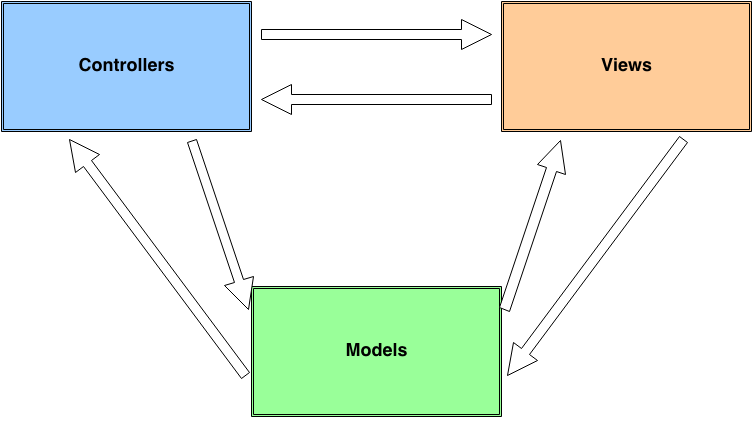
\includegraphics[height=3.5in]{figures/mvc.png}

    \caption[Model-View-Controller Architecture
    ]{A generic Model-View-Controller architecture.}

    \label{mvc}
\end{figure}

Controllers in AngularJS are stored as \emph{controllerName.js}. A controller in MVC is something that stores business logic that controls the web application. In AngularJS, any thing within the controller that is not a function will execute the moment that specific route is loaded. This includes any sort of models or JavaScript logic not wrapped in a function. Otherwise, the code within a function will not happen until that specific method is invoked. For example, all of the REST HTTP calls will happen right away when the controller is loaded.

Models in AngularJS are defined through the \$scope variable and are related to the variables that reside within the controller. The models are what contains data that is shown and also modified by the user. In the case of \projectName{}, these model data variables are usually data that \projectName{} queries from \ancor{}. An example of some of these data variables include instances, roles, and the \ancor{} version. AngularJS stores this data to make it easily accessible to the view.

Views in AngularJS are still in HTML, however developers are able to modify the DOM tags to contain Angular code that makes working with HTML a bit easier. The code segment in \ref{htmlcodefigure1} shows off an example of how AngularJS makes writing views easier. It is a code segment from \projectName{} where it builds a simple dropdown that contains all of the roles from \ancor{}. It gets the roles variable from the MainCtrl model and uses an AngularJS style for each to loop over all of the elements on roles to create a list of roles for the dropdown.

\begin{figure}[H]
  \begin{center}
    \renewcommand{\theFancyVerbLine}{
      \sffamily\textcolor[rgb]{0.5,0.5,0.5}{\scriptsize\arabic{FancyVerbLine}}}
    \begin{minted}[mathescape,
                   linenos,
                   numbersep=5pt,
                   gobble=2,
                   frame=lines,
                   framesep=2mm]{html}
    <ul class="dropdown-menu" role="menu" >
      <li ng-repeat="role in roles">
        <a ng-click="addNewRole(role)">
          {{role}}
        </a>
      </li>
    </ul>
    \end{minted}

  \end{center}
  \caption{AngularJS generating a dropdown menu.}
  \label{htmlcodefigure1}
\end{figure}

\subsection{Interacting with \ancor{} Through REST}

When \projectName{} needs to directly interact with \ancor{}, it communicates through a REST API, or Representational state transfer~\cite{DMatrix:Fielding:2000} API. Developed in 2000 by Roy Thomas Fielding, REST is a popular solution developers use when projects need to communicate to each other over HTTP.

By communicating over HTTP with REST, \ancor{} is able to expose a few functions that help outside users control the project. To start this process, you make an HTTP operation call to a specified URL. These operations are known as \emph{GET, POST, PUT,} and \emph{DELETE}. Since \ancor{} was designed to communicate to outside projects through REST, \projectName{} uses this API to send and receive data directly to \ancor{}. The following is a description of each component of the REST API basic functionalities with examples on how \projectName{} uses them.

\emph{GET} is a RESTful operation that when invoked, will return information depending on what endpoint has been queried. For example, if \projectName{} wants to get a detailed list of all the instances currently on \ancor{}, it can query the \emph{http://ancorIP/v1/instances} endpoint and get a json-formatted chunk of data that details all of the instances currently deployed.

\emph{POST} is a RESTful operation that allows information to be \emph{posted} to the remote server. This operation is often used when a website has form data that needs to be submitted to the remote server. In \projectName{}, \emph{POST} is used when a user is ready to submit a configuration file to deploy a new environment. In this case, we are not posted json formatted data to \ancor{}. In the header we put that the data is yaml format so \ancor{} knows what format to expect.

\emph{PUT} is a RESTful operation that implies that you are \emph{putting} or modifying a resource. This means you will replace whatever was there before with the new call. In \projectName{}'s case, this operation is used when we want to tell \ancor{} to commit the newly \emph{POSTED} environment.

\emph{DELETE} is a RESTful operation that will \emph{delete} a given resource depending on what endpoint is queried in \ancor{}. For example when a user wants to delete a given instance or an entire environment, they are able to make a \emph{DELETE} call to remove that given instance or environment.

\section{Use-Cases}
\label{makereference2.4}

In this section, I will describe the use-cases that this dashboard covers. These use-cases mirror the functionality of \ancorcli{}, but give a more visual interactive experience for the user instead of the terminal based experience \ancorcli{} gives.

\subsection{Viewing Instances}

The main use-case that this dashboard was developed for was seeing the state of instances from \ancor{}. This is also the main view of \projectName{} when you first visit the project in your browser. It displays how many instances \ancor{} currently has, as well as what current state each instance is in. If you scroll down, you can see the D3.js generated network graph. This graph displays the layout of \ancor{} and shows how each instance is related. This can be seen on figure \ref{mainInstanceView}. A closer look at the dynamically generated network graph can be seen in figure \ref{networkGraph}.

If a user wishes to see all of the instances of \ancor{} in more detail, they can scroll down to the table of instances near the bottom of the main page as seen in figure \ref{mainInstanceTableView}. In this case, the table shows the user the instance name, the interface it's on (an ip address), the current stage, and the planned stage. Clicking the more info button will display all of the relevant information that \ancor{} provides about each instance (figure \ref{modalInstanceView}). At the moment, there is no \ancor{} endpoint to query for any \emph{advanced} details, however there is a space left in case that feature is added in the future. The final column contains various operations that a user can perform on the instance as well.

If a user wants to search for something specific within the table, they are able to use the filter search box. As seen in figure \ref{instanceTableFilter}, when typing something in this box, the table will shrink down to match the search parameters.

\subsection{Viewing Tasks}

Visiting Tasks (figure \ref{tasksView}) will give you the state of all current tasks. They are sorted by tasks that were updated most recently and give a user an idea of what's currently happening on \ancor{}. For example, when a user deploys a new configuration, they are able to visit the tasks page to watch what tasks are currently in progress, what tasks have completed, or what tasks are suspended. They are also able to filter tasks if they are searching for something specific. The filter will work for any column in Tasks.

Like in the Main view, Tasks also has a filter search box to allow users to look through all Tasks. Typing anything in the search box will start the process of filtering through all of the Tasks data as seen in figure \ref{tasksFilter}.

\subsection{Deploying New Roles/Instances}

All roles can be discovered by selecting the dropdown link above the Instance overview table. Each element in the dropdown for adding a new role is the given role slug provided by \ancor{}. This dropdown can be seen in figure \ref{dropdownRoles}.

If a user wants to deploy a new role to \ancor{}, they can select one of the role slugs from the dropdown menu. \projectName{} will then make an HTTP POST call to \ancor{} with the selected role slug to deploy a new specified instance.

\subsection{Importing Configuration Specification Files}

\projectName{} provides an interactive method for deploying and importing configuration specifications. Visiting the Deploy endpoint for \projectName{} will load up the ACE embedded cloud editor (figure \ref{deployView}). This editor is fully featured and supports yaml syntax highlighting.

For the users convenience, \projectName{} provides two templates that can be inserted into the arml specification while they develop their configuration file (figure \ref{aceEditorSample}). The first one is the basic goal template that a user will have to make when starting a new configuration. The other template provided is a role template, which a user can insert after they have created a goal within the configuration specification. These templates provide some basic structure that a user can modify while developing their configuration specification.

If a user is confused on the structure of an configuration specification, they can select the help button on top of the ACE Editor (figure \ref{deployHelpView}), which will bring in a modal view explaining the structure as well as showing an example that they can use.

\subsection{Replacing and Deleting Instances}

For replacing an instance, \projectName{} provides a button on the main Instance table view that a user can select to perform the replace action (figure \ref{replaceDeleteInstance}). When the user selects replace, the view will invoke the replaceInstance method in the main controller with the given instance id. \projectName{} then does an HTTP POST call to \ancor{} against the id passed in from the view. At the moment, \ancor{} does not support replacing an instance. However the code is in place once this feature has been completed, and the only change required would be uncommenting out some code within the main controller.

Similar to replacement, \projectName{} provides a way for a user to delete instances as well. Selecting the delete button from the instance table list will invoke a function within the Main controller to do an HTTP DELETE call to \ancor{} with the provided id.

\subsection{Viewing Environments}

If a user would like to see if the current environment is locked, or if they are interested in the name of the current deployments environment, they can visit the Environments page of the dashboard (figure \ref{envView}). This view will also let the user know if the environment is currently locked. When an environment is locked, that means \ancor{} is currently working on a job and no other operations can occur.

\subsection{Deleting Environments}

When an \ancor{} user wants to completely remove an environment, they can visit the Environments page of the dashboard. This view provides a button that will completely remove the current deployment. After invoking this operation, the Tasks page will show the progress of removing the specific environment. The delete button will become disabled if the environment is locked.

\section{Interaction Diagrams}
\label{makereference2.5}

Interaction diagrams give a general overview of how a user might interact with the software the diagrams were based off of. In this section, I introduce \projectName{}s interaction diagrams based off of the use cases referenced in \ref{makereference2.4}.

In figure \ref{mainInterDiagram}, we have the interaction diagram for the Main, Env, and Task endpoints. The first event that happens is when a user visits one of the three endpoints on the dashboard. This will kick off a few HTTP GET calls which will interact with \ancor{}'s REST API. These HTTP GET calls are different depending on which endpoint we are looking at (this will be explained in the next chapter). Once the controller receives a response from \ancor{}, if successful, it will take the json data it received and store it in a model variable to be used for later. This model variable will also be displayed on the view for the user to see and interact with. If there are any updates made by the user through the view, those updates will also be made in the model because of AngularJS data binding. The views also have various functions that can interact with the controller. For example in the Main view, there are functions for creating and deleting instances. These functions are invoked from the controller, which then make the appropriate HTTP POST or HTTP DELETE calls to \ancor{}.

\begin{figure}[htb]%t=top, b=bottom, h=here

    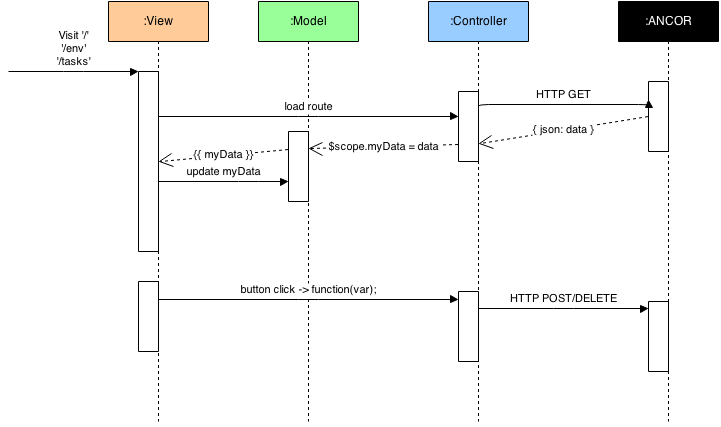
\includegraphics[height=3.5in]{figures/MainCtrl-Interaction-Diagram.png}

    \caption[Main, Env, and Task Interaction Diagram
    ]{Interaction diagram for Main, Environment, and Tasks endpoints.}

    \label{mainInterDiagram}
\end{figure}

In figure \ref{deployInterDiagram}, we have the interaction diagram for the Deploy endpoint. When this endpoint is first loaded up, it goes out and fetches environments from \ancor{}. This is so the user can be informed as to how many environments are currently deployed in \ancor{}. Currently, this is important because the dashboard only supports a single deployed environment. Next, the ACE editor is loaded up for the user to interact with. The user is able to have a full editor where they can write their configuration configuration file. As the user writes out their configuration, the View makes sure to update the model as to what is within ACE. Once the user clicks the deploy button, \projectName{} will take all of the text within the ACE Editor to send off to \ancor{}. It will first to an HTTP POST that contains the configuration data in yaml format. Once that call has been successful, it will do an HTTP PUT to let \ancor{} know to commit the changes and start the deployment.

\begin{figure}[htb]%t=top, b=bottom, h=here

    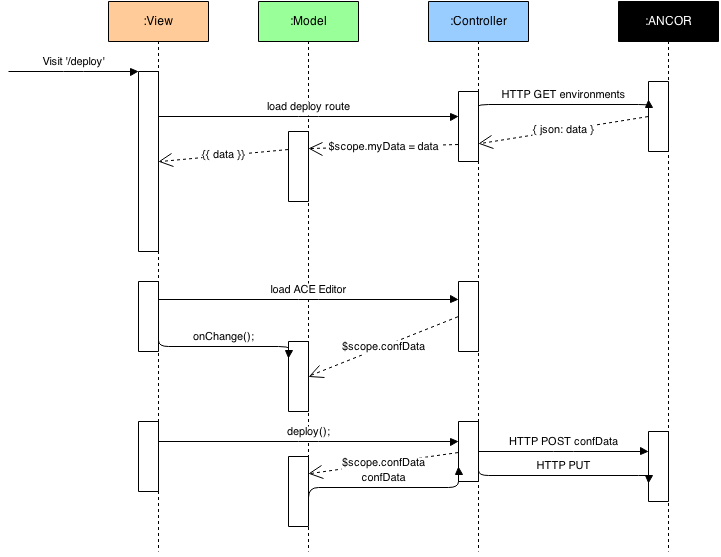
\includegraphics[height=4.5in]{figures/deploy-instance.png}

    \caption[Deploy Interaction Diagram
    ]{Interaction diagram for Deploy endpoint.}

    \label{deployInterDiagram}
\end{figure}

% +--------------------------------------------------------------------+
% |Chapter 3
% +--------------------------------------------------------------------+

\cleardoublepage

\chapter{\projectName{} Implementation}
\label{makereference3}

In this chapter, I will go over the main implementation details for the project. This will include the final architecture design, the original development process, a discussion on how some of the code has been implemented, and then a component breakdown of the entire project.

\section{Final Architecture and Design}
\label{makereference3.1}

For the final design of \projectName{} I choose the traditional Model-View-Controller architecture for a web application.

Following figure \ref{fullArchitecture}, we can see that we have \ancor{} as a black box that the \projectName{} communicates with. When \projectName{} needs to retrieve or send data to \ancor{}, it will send an HTTP GET, PUT, POST, or DELETE call to invoke a REST action. This is represented in the figure by the two arrows between the \ancor{} black box and the controller.

Within the dashed rectangle with rounded edges, I have represented \projectName{}. It follows the Model-View-Controller architecture that most web applications conform to. The controller is where all of the methods and HTTP REST functions are located. It is also the component in charge of defining the models. After a successful HTTP call from \ancor{}, the controller will save the relevant data into the model. On the view, if any of the model variables are needed, they can be accessed and displayed to the user. Also, if there are any functions that need to be called from the controller, the view contains buttons to invoke these functions.

Finally on the very right of figure \ref{fullArchitecture}, we have the user browser. This is where the user interacts with \projectName{}. Normally the user will retrieve the compiled template view that is ready to be displayed in the browser. However if the user wishes to add a new instance, delete an instance, deploy a new configuration file, etc, then they will invoke that action through the view that will then call a method within the controller.

\begin{figure}[htb]%t=top, b=bottom, h=here

    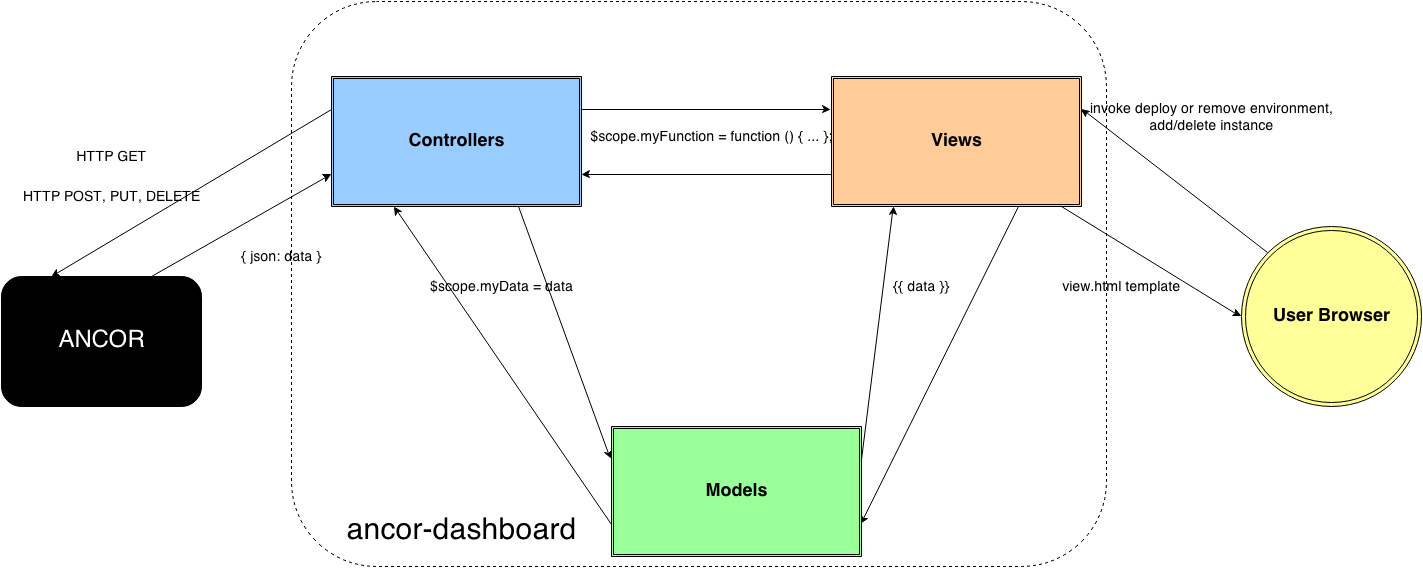
\includegraphics[height=2.8in]{figures/ad.png}

    \caption[\projectName{} Full Architecture
    ]{Full caption to appear below the Figure}

    \label{fullArchitecture}
\end{figure}

\section{Prototyping}
\label{makereference3.2}

Initially, this project was developed with Ruby on Rails. After a few months of development, it became clear that Ruby on Rails was a heavy framework to use for a project like this. Not only that, but because of the way Ruby on Rails works, it added an extra step to interact with \ancor{}. With Ruby on Rails, if a user wanted to make an API call to \ancor{} (like deploying a configuration file or viewing tasks), the user would have the browser talk to the Ruby on Rails server, and then that server would talk to \ancor{}. This added an extra step in the interaction between \projectName{} and \ancor.

To resolve this issue, I redid the framework in AngularJS. With AngularJS, the software is compiled to minified CSS and JavaScript and ran on the users machine directly. This compiled code will often be placed in an Apache or Nginx server to be served out to the user. In this case, there is no longer that extra medium required to talk to \ancor. Now the user can directly communicate with \ancor{} through their browser without needing to query a Ruby on Rails server first.

\section{\projectName{} Code Discussion}
\label{makereference3.3}

In this section, I will break down some of the major functionalities of \projectName{} and talk about how the code accomplishes those functionalities.

\subsection{REST over HTTP with AngularJS}

Earlier in chapter 2, I mentioned the idea of how \projectName{} communicates with \ancor{} with a concept called REST over HTTP. As mentioned before, REST has several different protocols to interface with: \emph{GET, PUT, POST, and DELETE}. But how exactly does that work within this project? Let's take a look at the Main controller to get a better idea of how this interaction works.

\begin{figure}[H]
  \begin{center}
    \renewcommand{\theFancyVerbLine}{
      \sffamily\textcolor[rgb]{0.5,0.5,0.5}{\scriptsize\arabic{FancyVerbLine}}}
    \begin{minted}[mathescape,
                   linenos,
                   numbersep=5pt,
                   gobble=2,
                   frame=lines,
                   framesep=2mm]{javascript}
    $http.get($rootScope.ancorIPAddress+'/v1').success(function(data) {
      $scope.version = data.version;
    });
    \end{minted}

  \end{center}
  \caption{\projectName{} using REST to ask \ancor{} what version it is.}
  \label{httpGET}
\end{figure}

\begin{figure}[H]
  \begin{center}
    \renewcommand{\theFancyVerbLine}{
      \sffamily\textcolor[rgb]{0.5,0.5,0.5}{\scriptsize\arabic{FancyVerbLine}}}
    \begin{minted}[mathescape,
                   linenos,
                   numbersep=5pt,
                   gobble=2,
                   frame=lines,
                   framesep=2mm]{html}
    <title>ANCOR {{version}} Dashboard</title>
    \end{minted}

  \end{center}
  \caption{Displaying a model variable within a view.}
  \label{modelView}
\end{figure}

In figure \ref{httpGET}, we have a simple HTTP GET call to \ancor{} that is retrieving the \emph{version} to display to the user on the dashboard. It queries the version number through a URL, and then \ancor{} responds with a json formatted data set. In this case, \ancor{} responds with the version number. In the controller we set that version to a model variable to be displayed on the view as seen in figure \ref{modelView}. The double brackets in AngularJS represent an evaluation. Because the variable version exists within the \$scope model, the view is able to display that value within HTML to the user. If no data is returned from \ancor{} in the controller,  the \emph{version} model variable will be empty and the evaluation will be left blank when the view is compiled.

\begin{figure}[H]
  \begin{center}
    \renewcommand{\theFancyVerbLine}{
      \sffamily\textcolor[rgb]{0.5,0.5,0.5}{\scriptsize\arabic{FancyVerbLine}}}
    \begin{minted}[mathescape,
                   linenos,
                   numbersep=5pt,
                   gobble=2,
                   frame=lines,
                   framesep=2mm]{javascript}
    $scope.addNewRole = function (roleSlug) {
      var url = $rootScope.ancorIPAddress+'/v1/instances',
          newRole = { 'role': roleSlug };
      $window.alert('New role ' + roleSlug + ' added!');
      $http.post(url, newRole);
      $route.reload();
    };
    \end{minted}

  \end{center}
  \caption{Code from the Main controller to add a new role to \ancor{} with an HTTP POST call.}
  \label{httpPOST}
\end{figure}

In figure \ref{httpPOST}, we have an example of an HTTP POST call to \ancor{}. In this case, this function is invoked when a user is interested in adding a new role through the role dropdown generated on the main page. First it builds the correct URL with a json data key value structure. It alerts the user that the invocation has started, and then sends the json data to the specified URL. \ancor{} will then take over from there, and the page is reloaded.

\subsection{D3 Network Graph}

On the main view of the dashboard, we have a dynamically generated network graph that uses D3js. This can be seen in figure \ref{networkGraph}. The initial graph drawing code was modified from one of the numerous D3js examples on the main website. However the code has been modified to work within the project itself. For example, to generate the nodes on the network, it must take a specially formed set of data from the Main controller. The main controller first does an HTTP GET call to retrieve all of the instances. Within this json on each instance, there is a \emph{depends\_on} attribute that is used to get what each node depends on and interacts with. A json object is then created with the source name, each sources dependency (or target in this case), the type of dependency (this will determine the color and style of the line with css), and the source ID. This data set is then passed into the method located in \emph{forced-graph.js} that generates the entire network graph.

The network graph code also defines how large each node circle will be, the length between connections, the color and size of the text used, and so on. Everything about the network graph is customizable here. Another modification to the network graph script was preventing the graph from jumping around when first loaded. Many D3js examples have very active elements when first loaded, almost like bouncy balls being released into a gymnasium. There is a simple method near the bottom that skips this activity so the graph looks more static on first load. This does not however prevent the user from dragging nodes around and moving the network graph on the page.

It has an event method for when a user selects one of the nodes. At the moment, this method only prints the node name and id to the JavaScript console. However in the future this method will be used for more than just that. See the future work section for more information.

\subsection{ACE Editor}

% image of ace editor?

The ACE Editor is an important part of the configuration writing process with \projectName{}. Thanks to the angular-ui library, integrating the ACE Editor is extremely easy. In figure \ref{aceEditorHTML}, we can see that adding a new editor is as easy as making a simple div tag with a few options defined. We give this div a specific id so that the controller knows which div to apply to.

\begin{figure}[htb]%t=top, b=bottom, h=here

    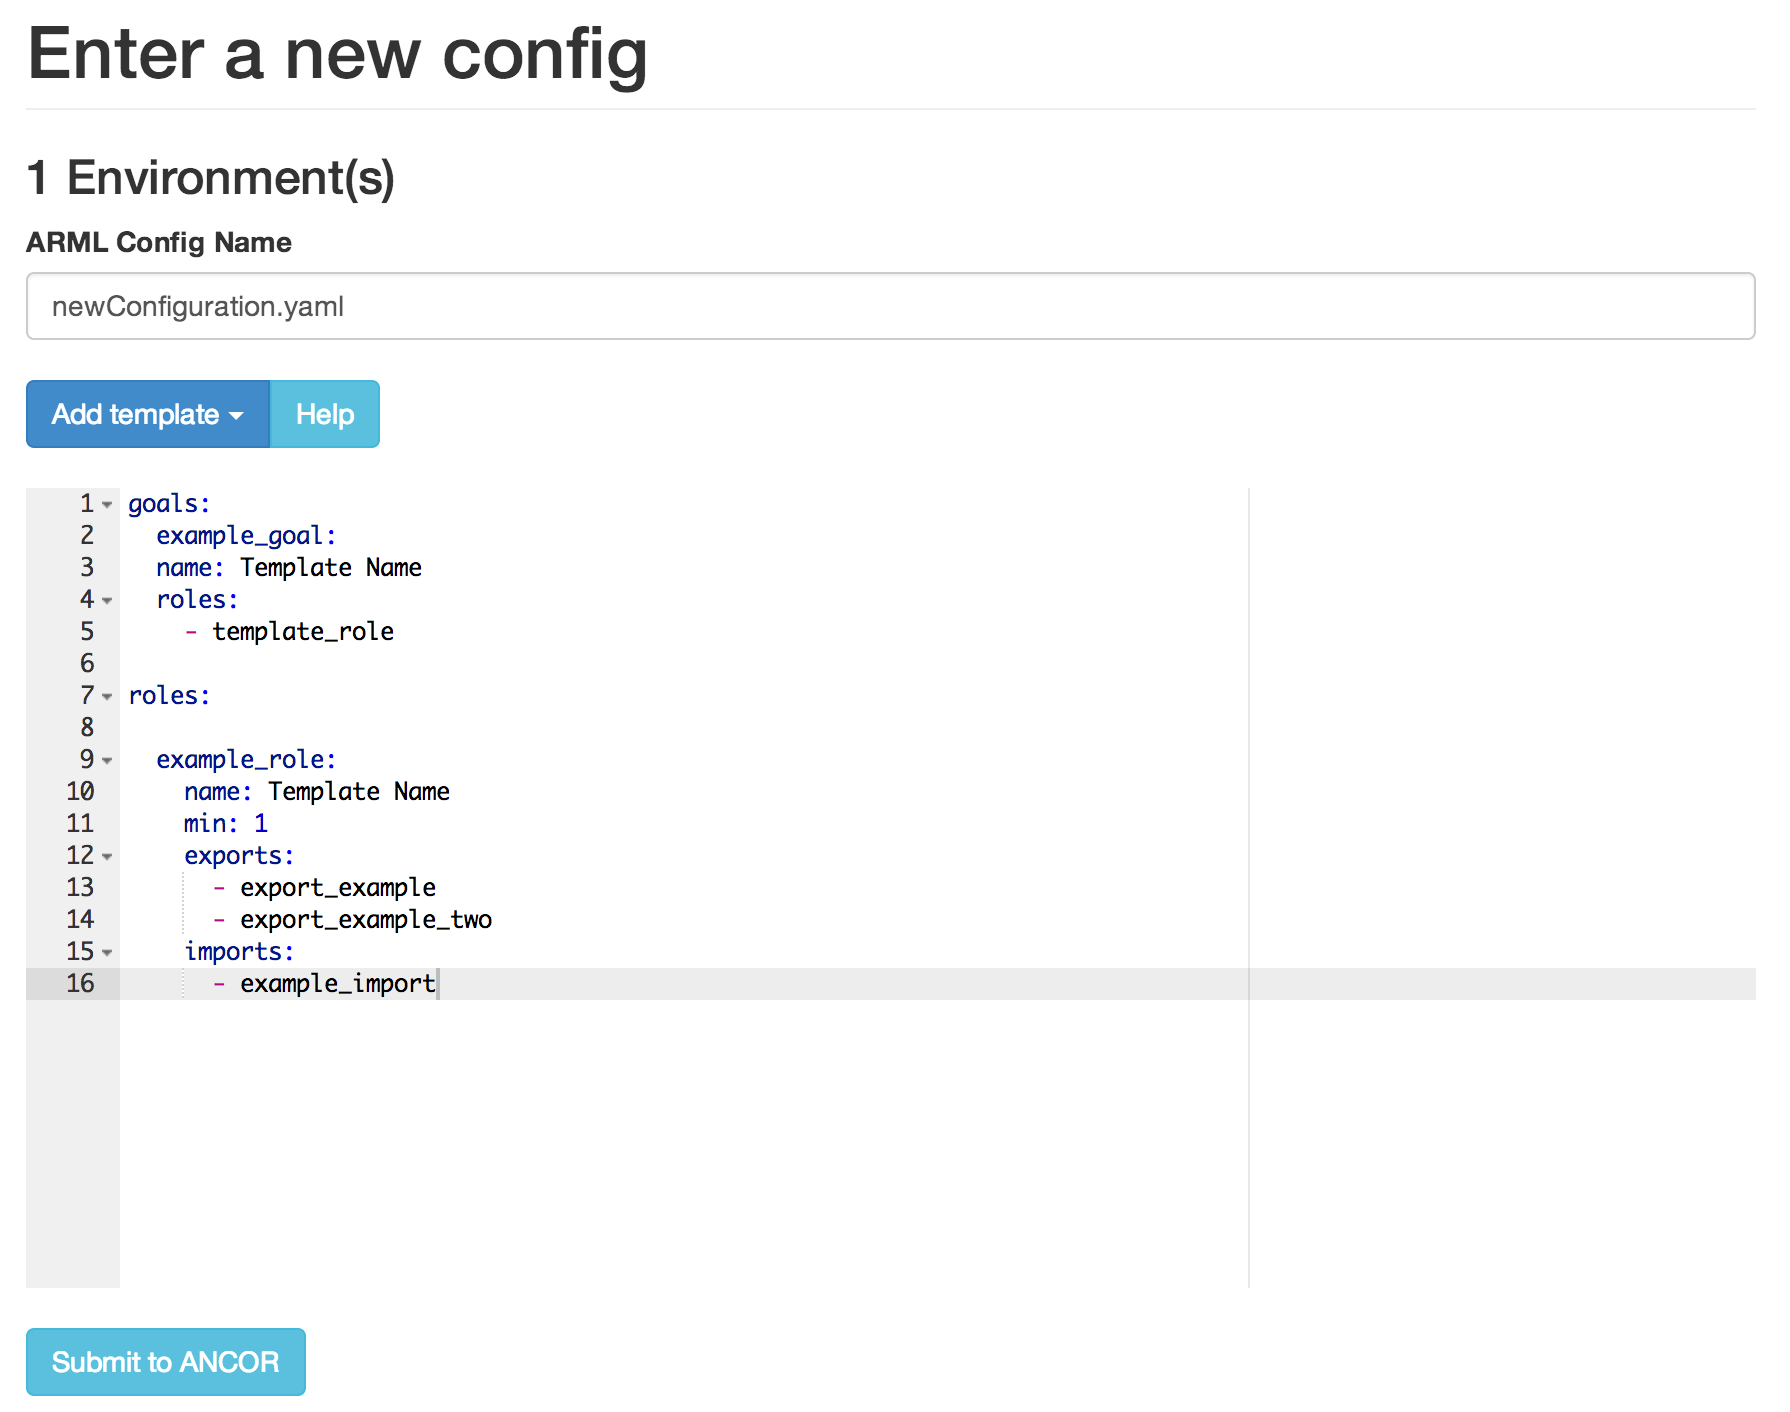
\includegraphics[height=5.0in]{figures/ace-editor-example.png}

    \caption[ACE Editor example
    ]{An example of what the ACE Editor looks like with a sample config file.}

    \label{aceEditorSample}
\end{figure}

Next with angular-ui, we pass in different configuration options to customize ACE. For example, the configuration files that \ancor{} uses are of the yaml syntax, thus we tell ACE to use yaml syntax highlighting for anything within the editor. useWrapMode is a standard text editing feature that prevents users from having to scroll side to side while typing up a document. Finally the two functions onLoad and onChange are functions defined by angular-ui's ACE package for when the editor first loads and when someone makes a change within the editor. These options are just the names of the functions from within the controller. An example of how the onChange and onLoad functions work can be seen in figure \ref{aceEditorOnChange}.

\begin{figure}[H]
  \begin{center}
    \renewcommand{\theFancyVerbLine}{
      \sffamily\textcolor[rgb]{0.5,0.5,0.5}{\scriptsize\arabic{FancyVerbLine}}}
    \begin{minted}[mathescape,
                   linenos,
                   numbersep=5pt,
                   gobble=2,
                   frame=lines,
                   framesep=2mm]{html}
    <div id="editor" ui-ace="{
      mode: 'yaml',
      useWrapMode: true,
      onLoad: loadConf,
      onChange: confChange
      }">
    </div>
    \end{minted}

  \end{center}
  \caption{Initializing the ACE Editor with angular-ui.}
  \label{aceEditorHTML}
\end{figure}

\begin{figure}[H]
  \begin{center}
    \renewcommand{\theFancyVerbLine}{
      \sffamily\textcolor[rgb]{0.5,0.5,0.5}{\scriptsize\arabic{FancyVerbLine}}}
    \begin{minted}[mathescape,
                   linenos,
                   numbersep=5pt,
                   gobble=2,
                   frame=lines,
                   framesep=2mm]{javascript}
    $scope.loadConf = function(_editor) {
      var _session = _editor.getSession();
      _session.setUndoManager(new ace.UndoManager());
    };

    $scope.confChange = function(e, _editor) {
      $scope.submitData = _editor.getValue();
    };
    \end{minted}

  \end{center}
  \caption{Two examples that help operate the ACE Editor. loadConf is what initializes the editor, while confChange keeps the configuration model variable up to date as a user writes their configuration file.}
  \label{aceEditorOnChange}
\end{figure}

\subsection{Table Filtering with AngularJS}

One of the advantages of using AngularJS is how simple they have made implementing complex features in HTML and JavaScript. One example of this is the search box that exists on the Main and Tasks view for filtering the large tables of data from \ancor{}. This consists of only a few components in the HTML template. The first one is the textbox. From figure \ref{filterTextSearch}, you can see the input text box tag with an ng-model attribute. This model variable is what keeps track of the input from the user.

The only other element to this powerful search function is the filter attribute when AngularJS builds the Task or Instance rows within the table. Looking at line 5 of figure \ref{filterTextSearch}, the final element in ng-repeat is \emph{filter:searchText}. This means if a user starts typing and modifying the model searchText, it will filter the results in the table automatically. This is a very powerful feature that only required a few lines of code thanks to AngularJS.

\begin{figure}[H]
  \begin{center}
    \renewcommand{\theFancyVerbLine}{
      \sffamily\textcolor[rgb]{0.5,0.5,0.5}{\scriptsize\arabic{FancyVerbLine}}}
    \begin{minted}[mathescape,
                   linenos,
                   numbersep=5pt,
                   gobble=2,
                   frame=lines,
                   framesep=2mm]{html}
    . . .
    <input type="text" placeholder="Search tasks..." 
      class="form-control" ng-model="searchText" />
    . . .
    <tr ng-repeat="task in tasks | orderBy:predicate:reverse | filter:searchText">
    . . .
    \end{minted}

  \end{center}
  \caption{An example of how AngularJS easily creates a filtering search box within a template view.}
  \label{filterTextSearch}
\end{figure}

\section{Component Breakdown}
\label{makereference3.4}

In this section, I will talk about the different components of \projectName. I will cover everything that exists in the controller as well as the viewmodel for each component.

\subsection{Main}

The main component of \projectName{} is the root route of the project. This means when a user first visits the main URL for \projectName{}, they will be presented with this view. This is the view in charge of displaying information about instances from \ancor{}. Once a user visits Main, the controller will then query \ancor{} through REST for its current version, all of the goals, all of the roles, and all of the instances.

These HTTP GET calls will then save the relevant information in the \$scope model for the view to use. Querying goals will get the name of the current deployment. This name is saved and shown as a title on the front page. Roles are queried for the add instance dropdown. Each role slug is saved so a user can select one from a dynamically generated dropdown.

With the call against \ancor{} instances, there is a bit of extra logic to keep track of each instances current stage and planned stage. The current stage is what is displayed to the user on the front page. It also shows how many total instances there are. Finally, data is saved and sent to the network graph generation script. This information is a set of data that shows how all of the instances are related to each other.

Two functions exist in this controller to replace and delete instances. They both are given an instance id, form the correct URL, and then make the appropriate REST HTTP call (either POST or DELETE) to \ancor{}.

There is a helper function to determine which label to apply to an instances state from the Instance table. This is needed so that the HTML template file can stay as simple as possible and let the controller do all of the logic for which class label to apply.

Finally, there are several functions in charge of showing the modal popup when a user is interested in viewing more information about each instance. These modal functions are mostly used by angular-ui's Bootstrap package.

\subsection{Env}

The Environment component is used to show the current deployment from \ancor{}. When this route is first loaded, the controller queries \ancor{} for its version and all of the current environments. At the moment, \projectName{} only supports one deployment, so we grab the first environment in the data returned.

The main function in this controller is the ability to delete the given environment. When the user clicks the delete button from the view, it passes the environment id to the controllers \emph{deleteEnv} function. This function then builds the correct URL with the id appended onto the end, and makes the HTTP DELETE call to \ancor{}.

Environment also has a helper function to determine if the delete button should be disabled or not. If the environment is locked, the button will become greyed out so the user cannot click on it. Otherwise, the button will be enabled.

\subsection{Tasks}

The Tasks view is what is in charge of displaying all current \ancor{} Tasks. When the Tasks view is first loaded up by the user, the controller then queries \ancor{} for its current version and all of the tasks. The HTTP GET for Tasks is different from other controllers however because it needed to be able to be refreshed constantly so a user could see the tasks progress. For this to happen, the HTTP GET call was wrapped up in a function within the controller. However since there is a call to that function \$scope.getData(), it is invoked initially when the route is loaded. Another way to update the task list is to select the \emph{Refresh} button located right above the filtering search box. Finally like the other endpoints, Tasks has a helper function to determine the label for each Tasks state.

\subsection{Deploy}

The Deploy view is where the user can write their own configuration file and deploy it directly to \ancor{}. When the Deploy route is loaded, it will query \ancor{} for its version and the current deployed environment. The environment is required just so the user can know if any environments are currently deployed to prevent any overlap.

roleTemplate and goalTemplate are what generates the template text for the configuration within the ACE Editor. It simply uses an already made string template and inserts it where the cursor is at within ACE.

There are two functions that relate directly to the ACE editor API. The first one is loadConf, which is in charge of initializing the editor. The next one is called confChange. This function is in charge of keeping the configuration data model up to date within Deploys model.

The deploy function takes the current data from the ACE editor and constructs a message to be sent off to \ancor{}. Before this happens, it builds two urls: A URL for planning the new deployment which will contain all of the configuration file data, and a URL for telling \ancor{} to begin the deployment. Once these URLS are created and the configuration data is saved, the deploy function makes these two HTTP PUT and POST calls (in that order) to \ancor{}.

The modal for Deploy uses all of the angular-ui conventions for displaying a modal to the users. It displays an example configuration, and gives some help text to help the user understand how to write a configuration file.

% +--------------------------------------------------------------------+
% | Chapter 4
% +--------------------------------------------------------------------+

\cleardoublepage

\chapter{Evaulation of Dashboard}
\label{makereference4}

\section{\projectName{} Evaluation}
\label{makereference4.1}

With the implementation of \projectName{} complete, there needed to be some testing to ensure that the dashboard was easy to use and as helpful as the \ancorcli{}.

\subsection{Speed}

\projectName{} is very fast and responsive in most modern web browsers. Because of the Bootstrap framework, it can work in the majority of what users will choose as their favorite browser. Since AngularJS compiles all of its HTML, CSS, and JavaScript down to a minified version, loading up the dashboard will be extremely fast when deployed. Because of how AngularJS is deployed, it will also be faster to respond compared to other popular MVC frameworks like Ruby on Rails or .NET as explained in section \ref{makereference3.2}, Prototyping.

\subsection{Usability of \projectName{} vs \ancorcli{}}

This project originally set out to cover all of the use-cases (section \ref{makereference2.4}) defined by the developers of \ancorcli{}. Because of this, \projectName{} is able to do everything that the \ancorcli{} can do. Since \projectName{} is a web application, it has an easier time displaying relevant information to the user compared to the \ancorcli{}. In \ancorcli{}'s case, the best it can do is display the json data in formatted tables within a terminal. This is just the nature and limitation of console applications compared to web application frameworks with rich visuals and point-and-click functionality.

\subsection{Using \projectName{} to Control \ancor{}}

Finally, \projectName{} should be able to control \ancor{} in such a way that it takes complete advantage of the REST API it has provided to interact with. With the addition of the powerful ACE Editor, AngularJS components like HTML templating to display relevant data, filtering to search through large data sets, dynamically generated network graphs, and other usability operations against \ancor{}, a user is able to do whatever they could need to accomplish with \projectName{}.

\section{Future Work}
\label{makereference4.2}

In this section, I will briefly go over some future work that could be done to the dashboard that would improve the user experience.

Eventually \ancor{} is planning on creating authentication for their REST API. When this happens, it will be important for \projectName{} to also have a way to authenticate users.

At the moment, if communication goes wrong with \ancor{}, there is not an intuitive way to let the user know. Errors will be displayed within the JavaScript console of a browser, however the average user will not think to look there if something unusual happens. It would be nice to give more feedback to the user when RESTful operation errors occur.

The instance network graph can also be improved to make it more helpful to the user. One improvement that could help is making the node links toggle between hidden and visible. Currently, there is no logic within the D3js script that keeps track of each nodes links once they are drawn. They all belong the the same CSS class. An improvement might be to separate each nodes links into different CSS classes, and then when a user clicks on a node toggle the CSS of its links between hidden and visible. This might make analyzing the network graph a little easier.

A usability improvement could be made to the tables in the Main and Tasks view. Adding a sortable toggle between each column attribute would improve how a user might go about looking at the data from \ancor{}.

% +--------------------------------------------------------------------+
% | Chapter 5
% +--------------------------------------------------------------------+

\cleardoublepage

\chapter{Conclusion}
\label{makereference5}

In this report, I have presented \projectName{}, a front end web application dashboard that interacts with the \ancor{} project. Built with the latest web technologies, \projectName{} is a powerfully light tool that makes using \ancor{} easier. Designed with the intention of replicating all of the functionalities that the \ancorcli{} provides, combined with the visual advantages that a dashboard provides, \projectName{} helps \ancor{} users be more productive and gives them a new experience when looking at the state of their deployed IT system.

\section{Source Code}
\label{makereference5.1}

The complete source code is currently located on a public repository on Github. The URL can be found below:

\begin{list}{-}{}
\item \url{https://github.com/arguslab/ancor-dashboard}
\end{list}

The repository offers a quick start guide for those wishing to contribute or test out \projectName{}. It also provides the binary files required for users to deploy within an Apache or Nginx deployment. This is provided so users will not have to install all of the dependencies needed to run the project locally.


% +-------------------------------------------------------------------------+
% | References                                                              |
% +-------------------------------------------------------------------------+

% +-------------------------------------------------------------------------+
% | In order for WinEDT to index references correctly, it has to know where |
% | the file resides.  The following command is prefaced by %, and will be  |
% | ignored completely by LaTeX.  However, WinEDT will use this line to     |
% | access the external .bib bibliography file.  Also note that WinEDT can  |
% | read file path names with either "\" or "/" - LaTeX, however, doesn't   |
% | like "\", so it's easier to store a path name in the "Unix" style.      |
% +-------------------------------------------------------------------------+

%Included for Gather Purpose only.  Do NOT uncomment:
%input "references.bib"

% +--------------------------------------------------------------------+
% | This template uses the BibTeX program to format references.  The
% | lines below create a separate Bibliography section and add
% | an entry for "Bibliography" to the Table of Contents.  The actual
% | data for your references (author, title, journal, date, etc.) are
% | entered in the references.bib file.  See that file for information
% | on how to enter references.
% +--------------------------------------------------------------------+

\cleardoublepage
\phantomsection
\addcontentsline{toc}{chapter}{Bibliography}
\bibdata{references}
\bibliography{references}

% +--------------------------------------------------------------------+
% | Finally, we generate the appendix.  To add or delete appendices,
% | add or remove the line
% |
% |     \input{appendixX.tex}
% |
% | where "X" is the letter designation of the Appendix (A, B, C, etc.)
% | You should have one \input{appendixX.tex} line and a corresponding
% | file appendixX.tex for each appendix.                                 |
% +--------------------------------------------------------------------+

\appendix
% +--------------------------------------------------------------------+
% | Appendix A Page (Optional)                                         |
% +--------------------------------------------------------------------+

\cleardoublepage

\chapter{\projectName{} Use-Case Screenshots}
\label{Appendix:Key1}

\begin{figure}[htb]%t=top, b=bottom, h=here

    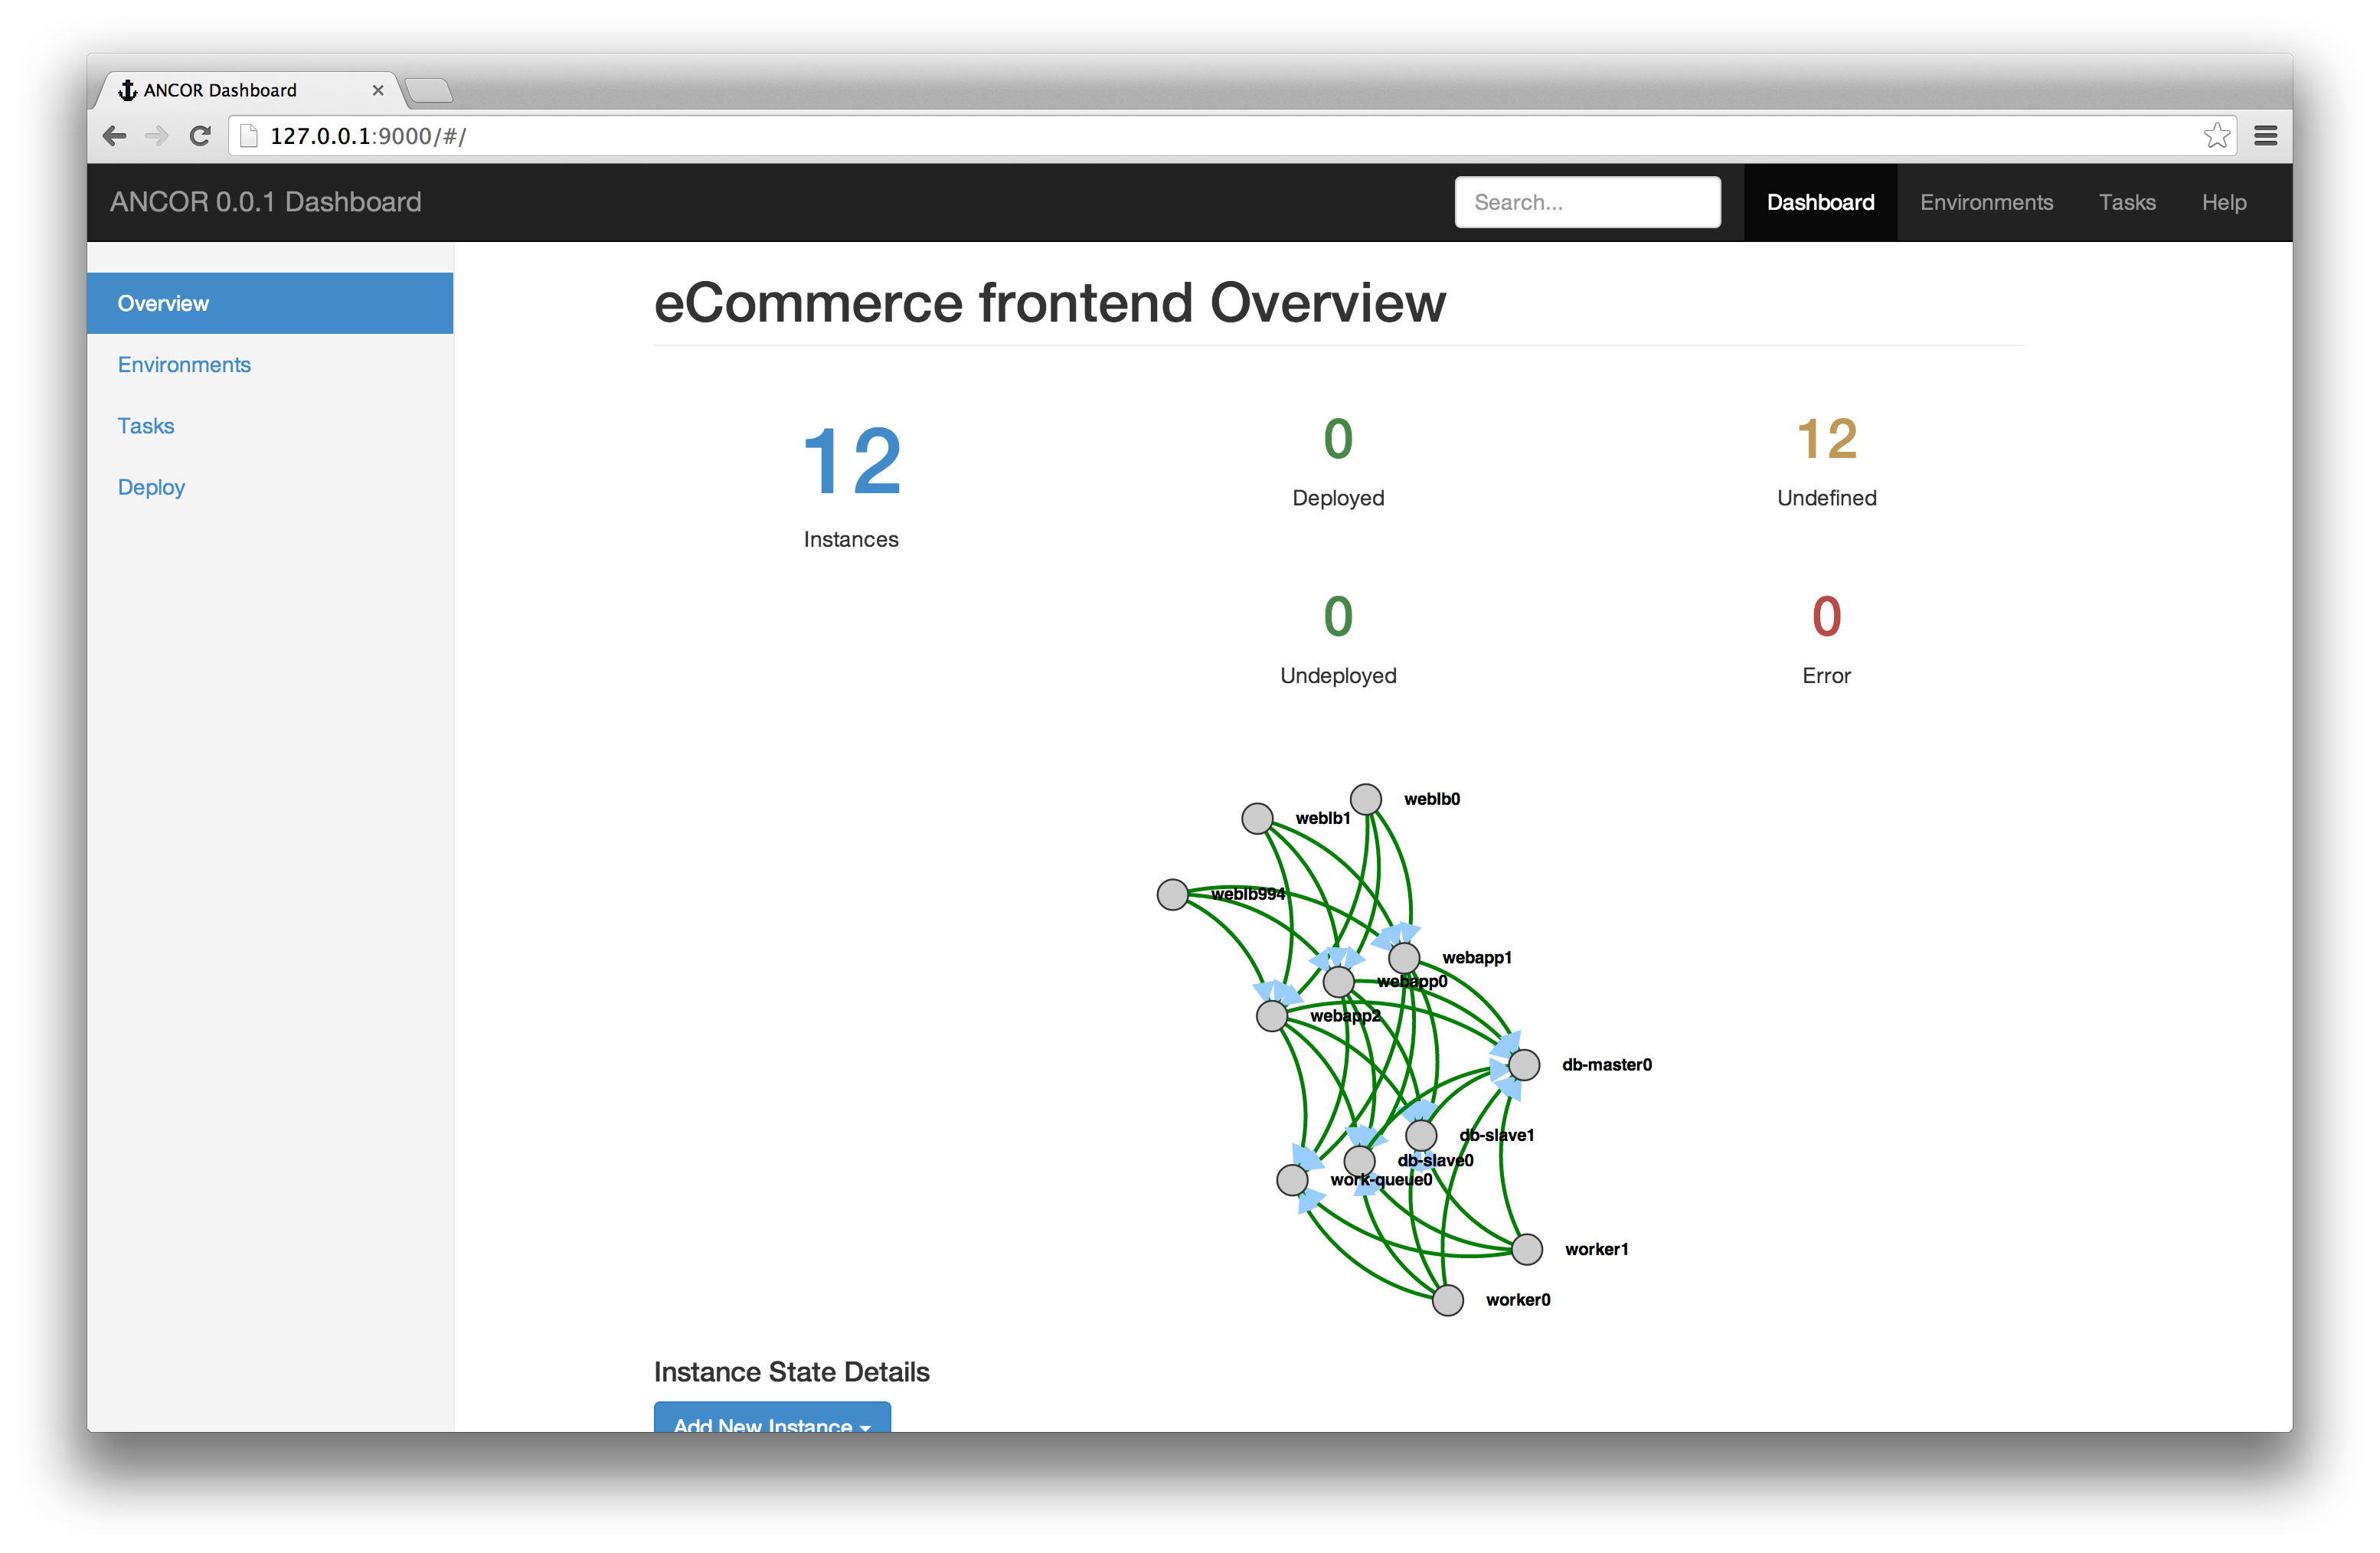
\includegraphics[height=4.0in]{figures/viewing-instances-main.png}

    \caption[The main view of a deployed ANCOR system.
    ]{The main view of a deployed ANCOR system.}

    \label{mainInstanceView}
\end{figure}

\begin{figure}[htb]%t=top, b=bottom, h=here

    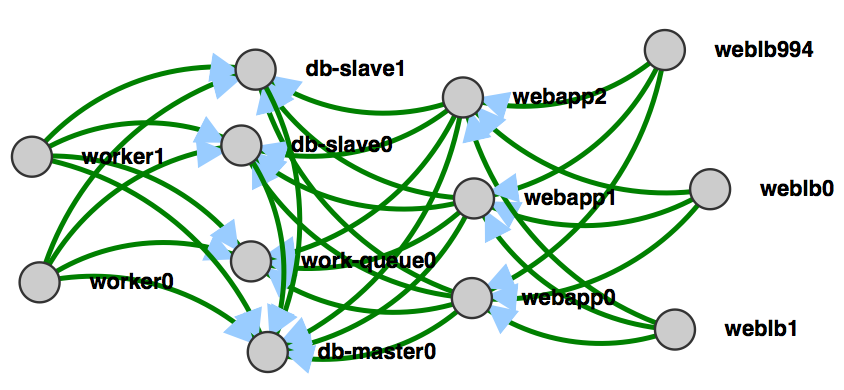
\includegraphics[height=3.0in]{figures/network-graph.png}

    \caption[D3.js Network Graph
    ]{A dynamically generated network graph.}

    \label{networkGraph}
\end{figure}

\begin{figure}[htb]%t=top, b=bottom, h=here

    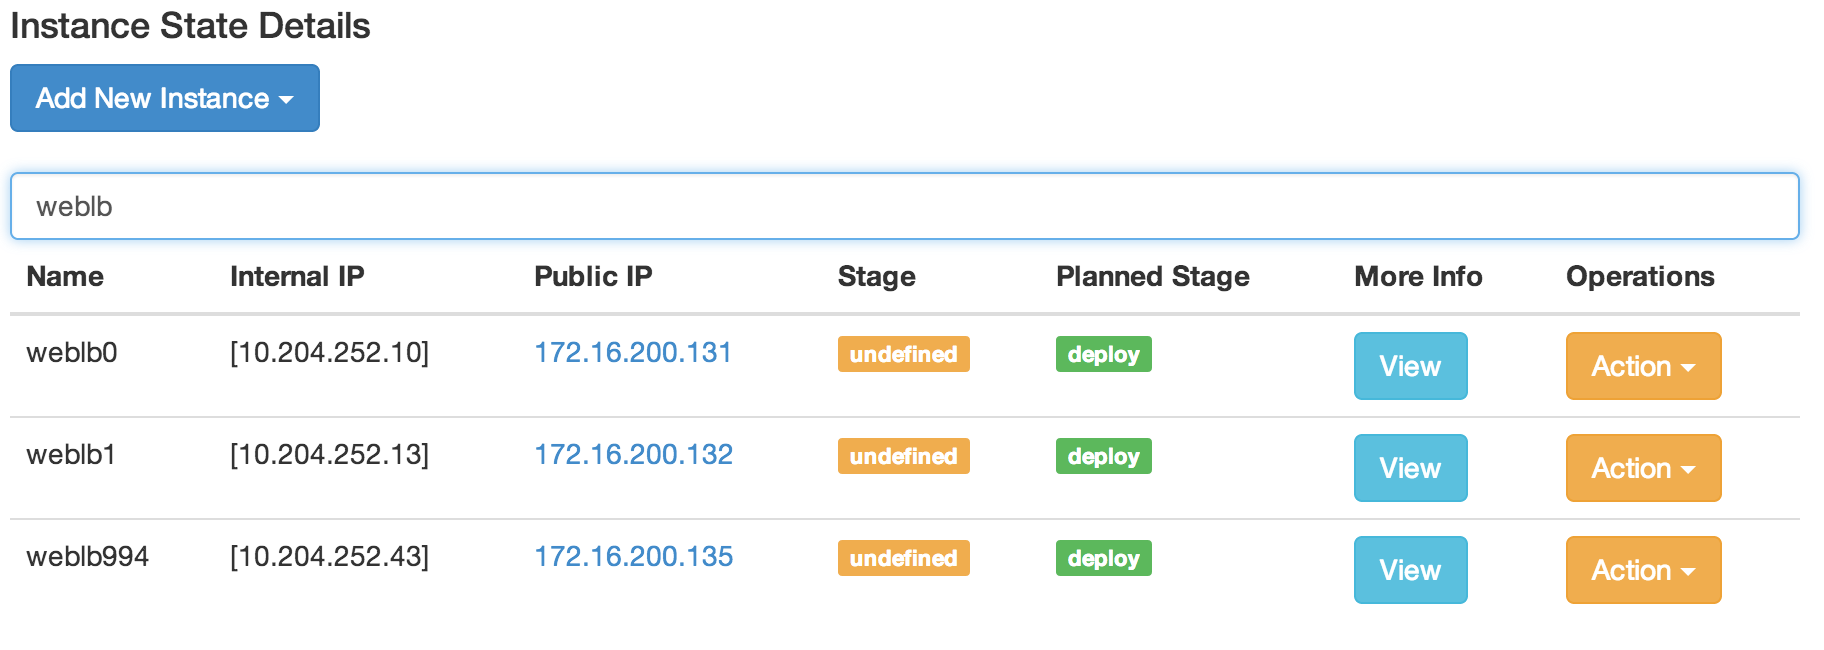
\includegraphics[height=2.3in]{figures/instance-table-filter.png}

    \caption[A user searching for weblb from the instance table.
    ]{A user searching for weblb from the instance table.}

    \label{instanceTableFilter}
\end{figure}

\begin{figure}[htb]%t=top, b=bottom, h=here

    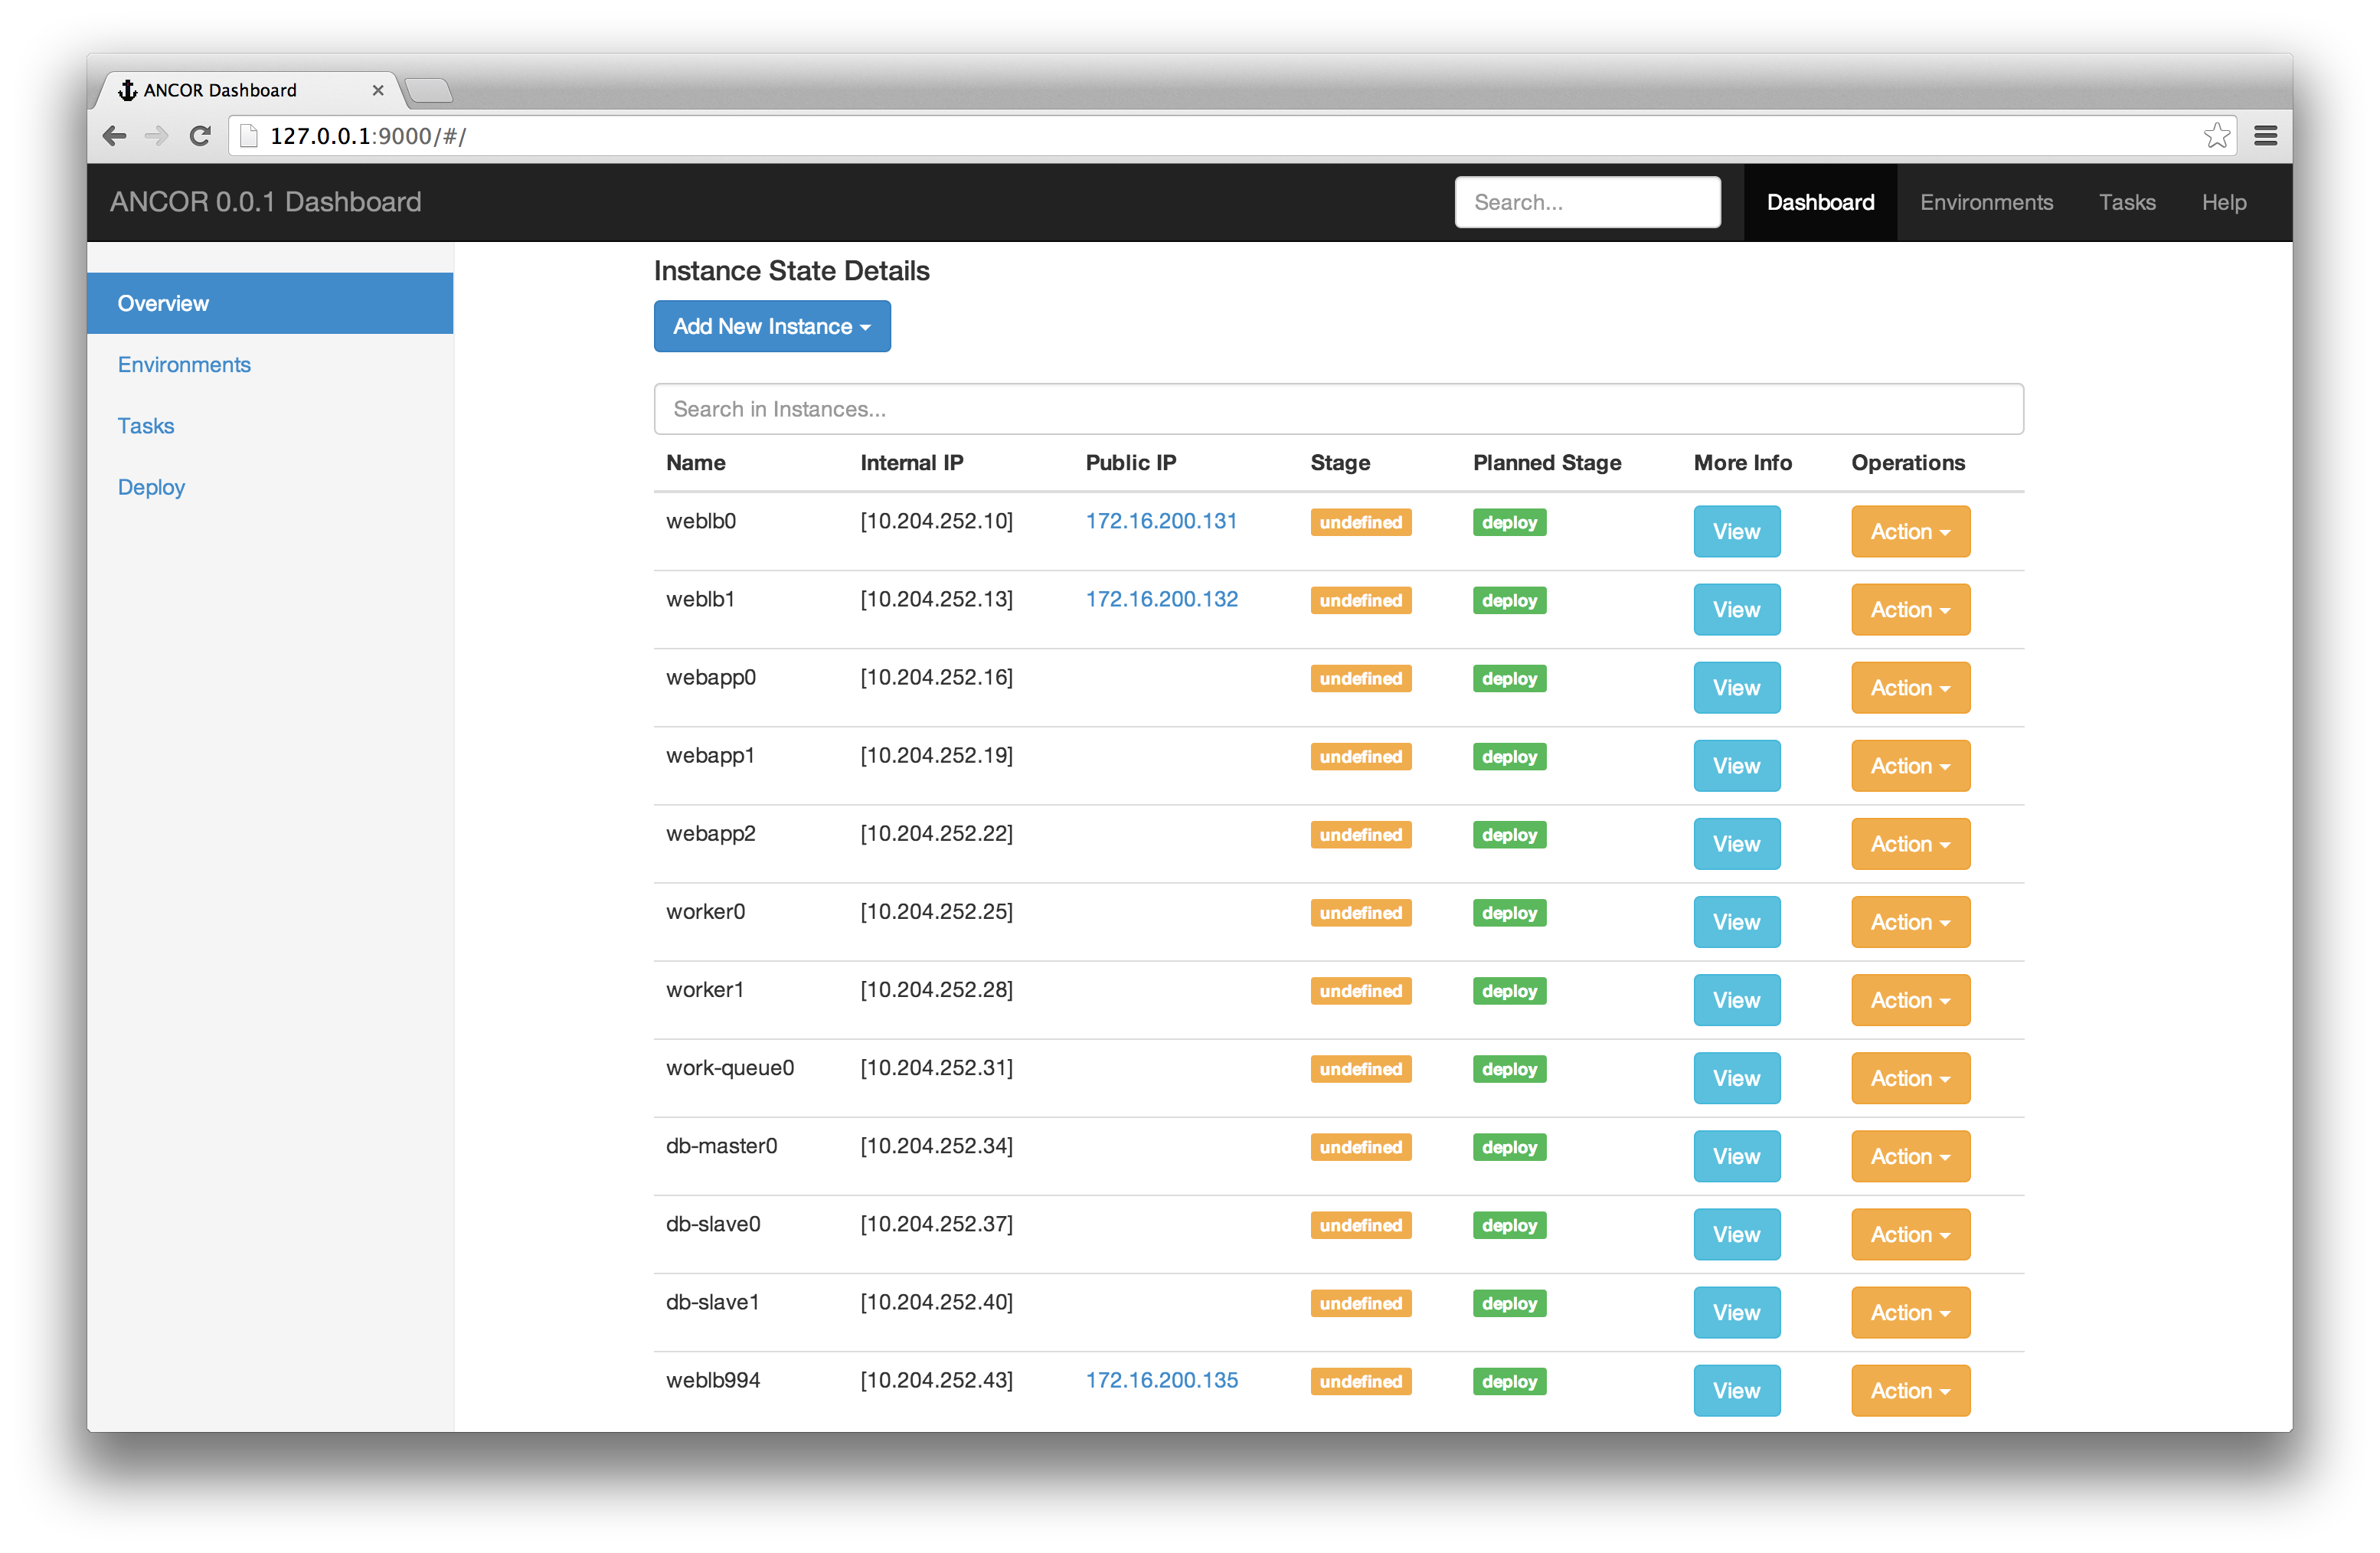
\includegraphics[height=4.0in]{figures/instance-table-view.png}

    \caption[Instance table view.
    ]{The instance table shown on the main view.}

    \label{mainInstanceTableView}
\end{figure}

\begin{figure}[htb]%t=top, b=bottom, h=here

    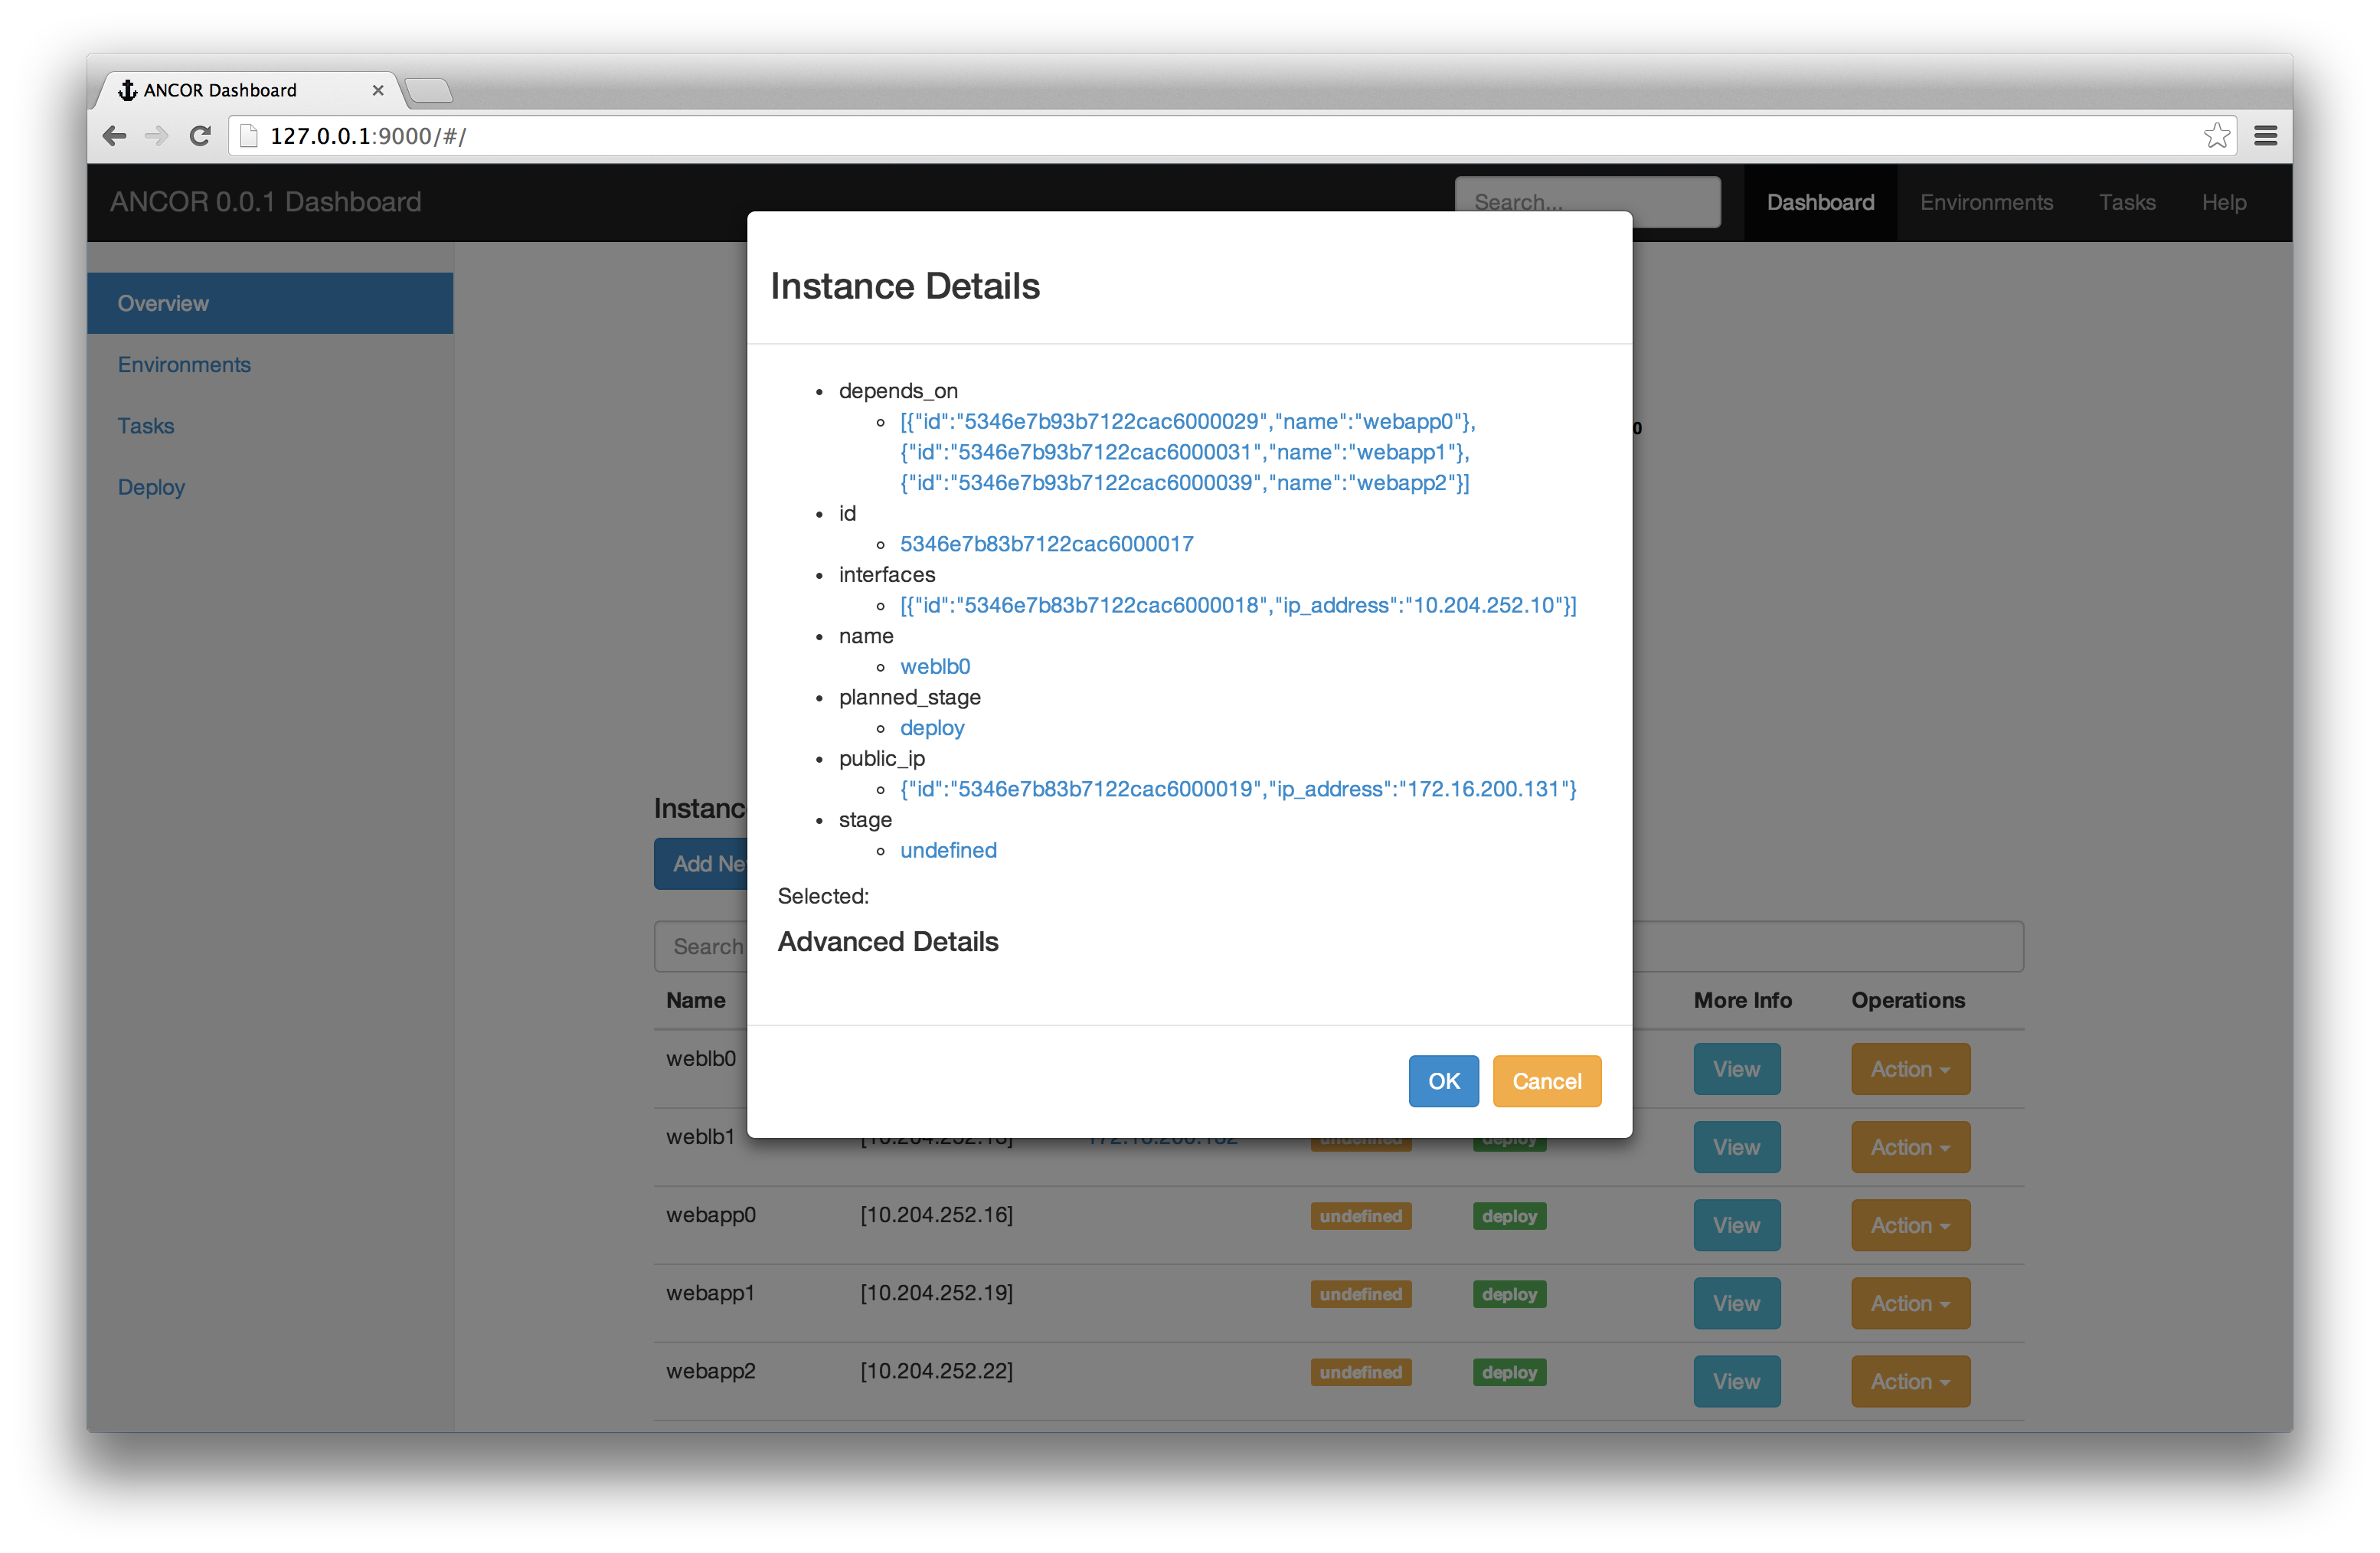
\includegraphics[height=4.0in]{figures/instance-modal-view.png}

    \caption[Instance modal view.
    ]{The instance modal view shown when a user wants more information.}

    \label{modalInstanceView}
\end{figure}

\begin{figure}[htb]%t=top, b=bottom, h=here

    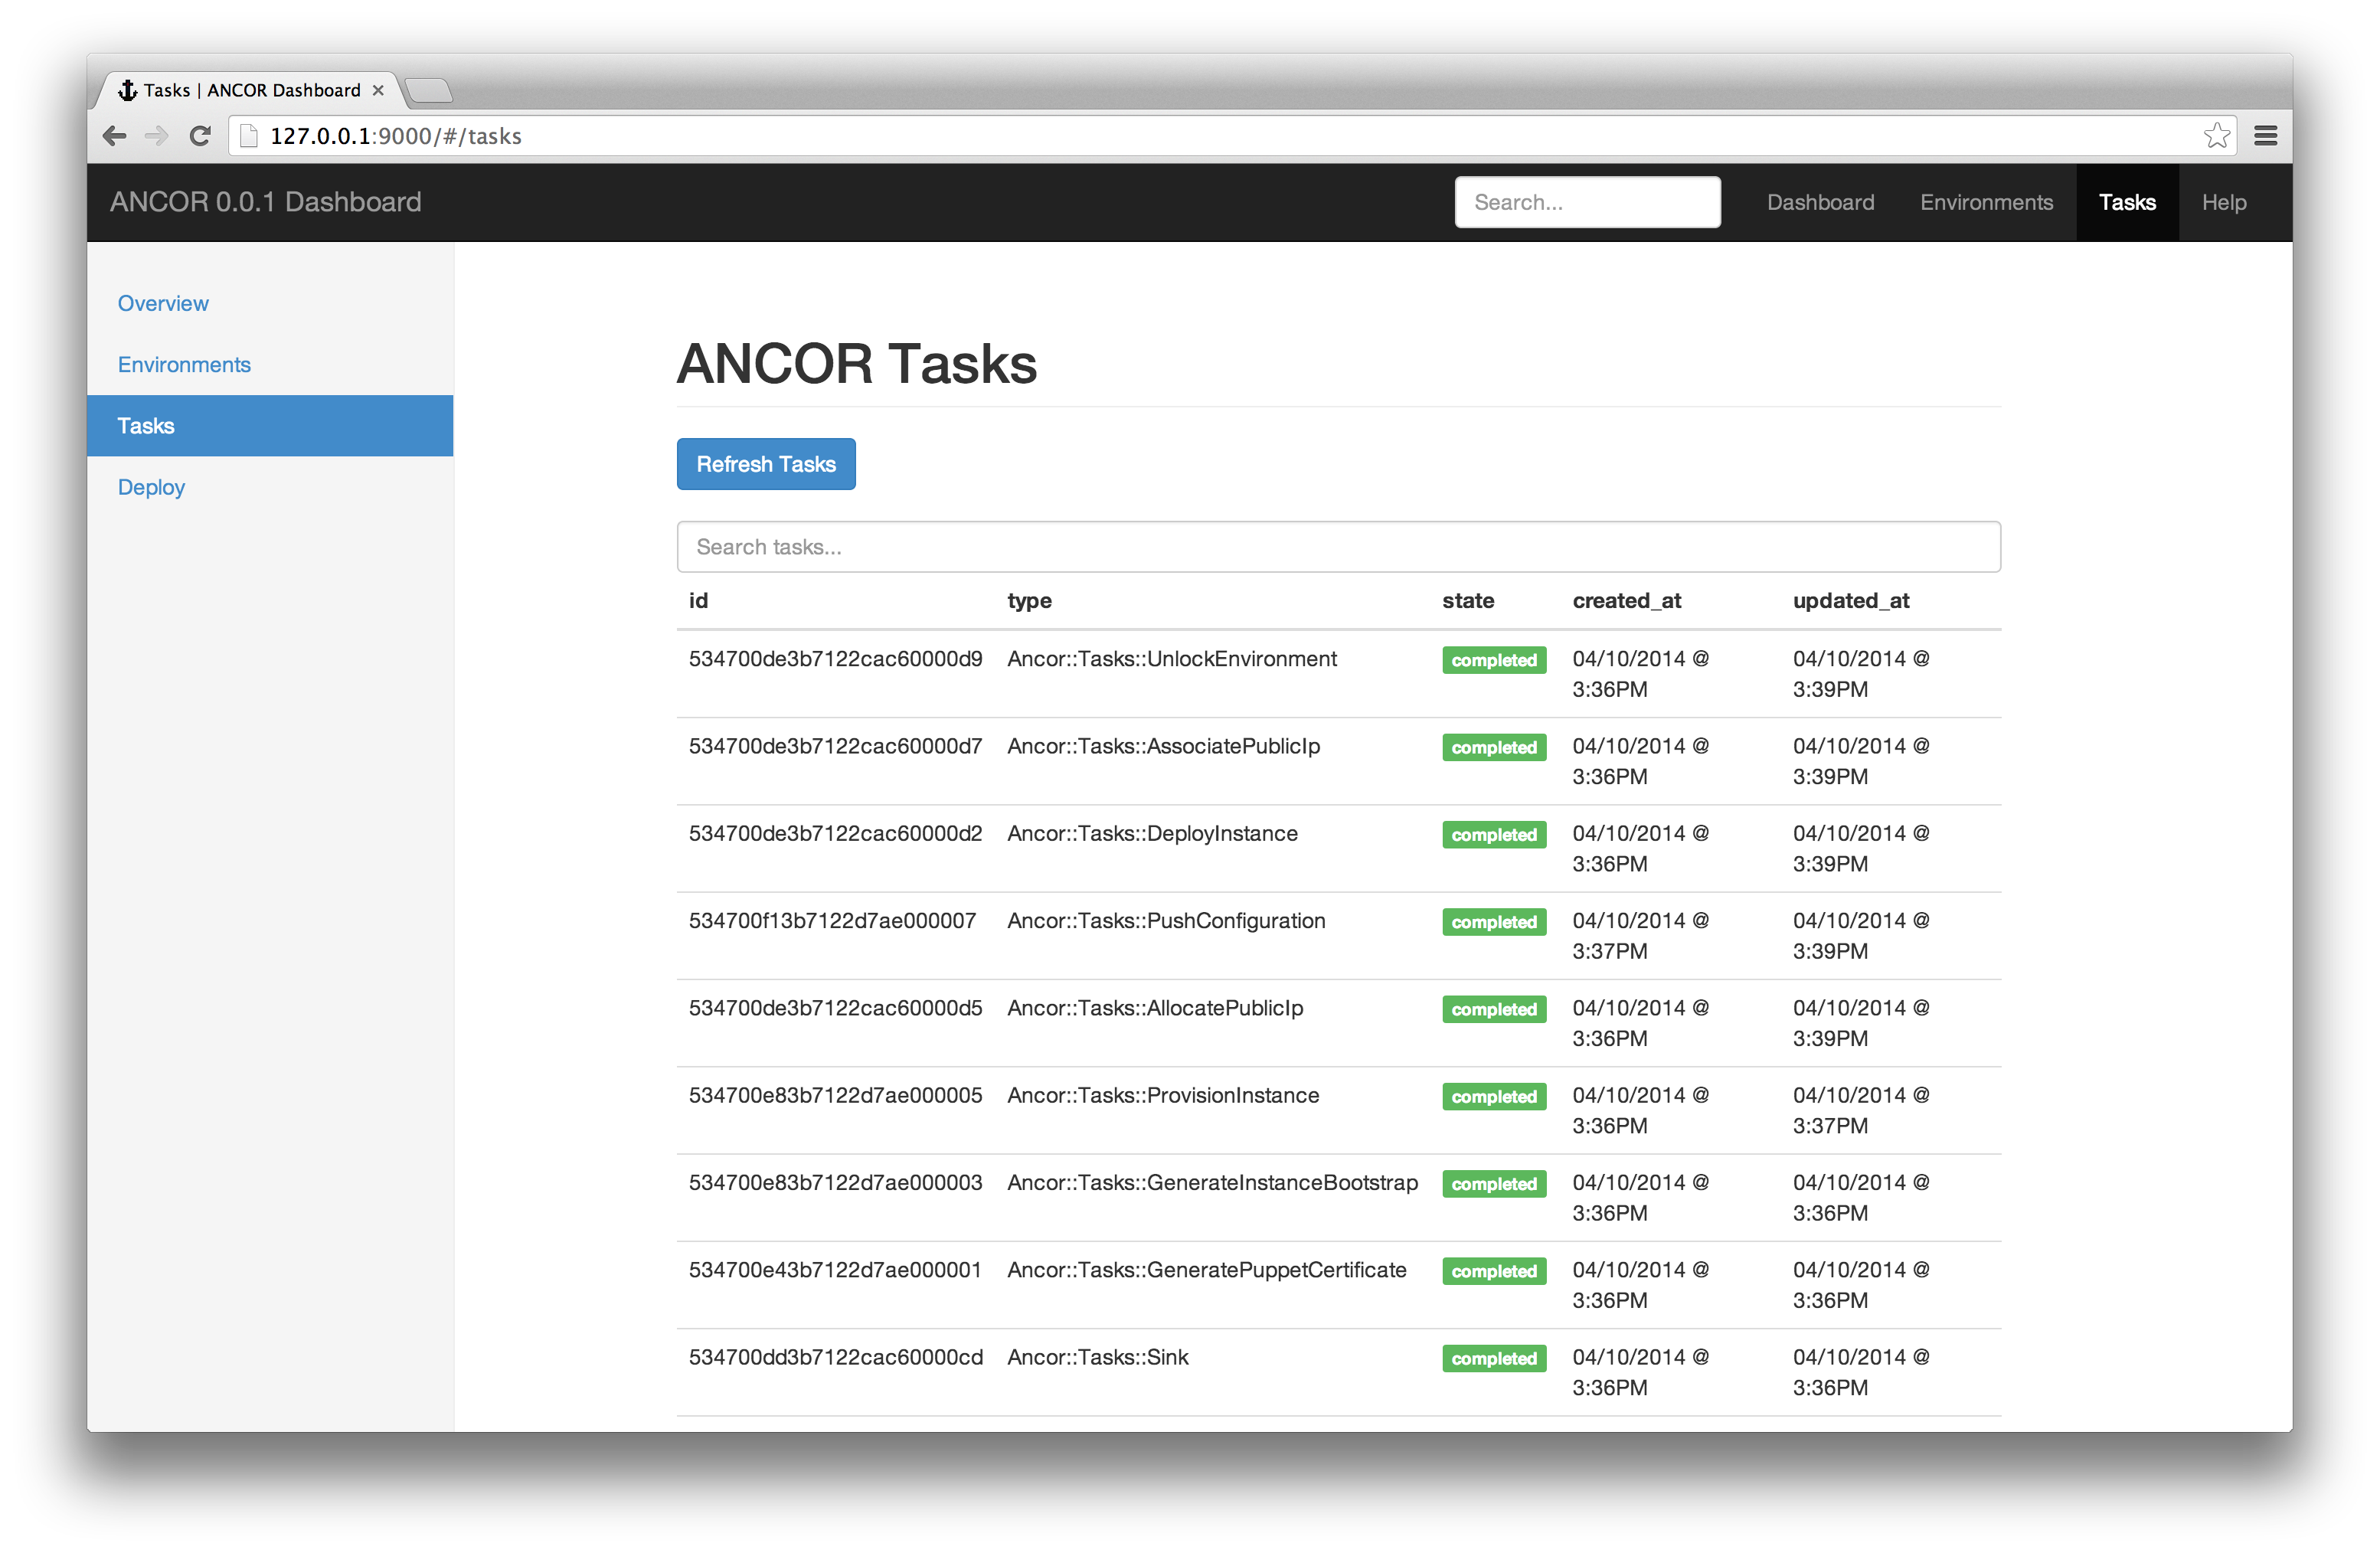
\includegraphics[height=4.0in]{figures/tasks.png}

    \caption[Tasks view.
    ]{A list of all current Tasks.}

    \label{tasksView}
\end{figure}

\begin{figure}[htb]%t=top, b=bottom, h=here

    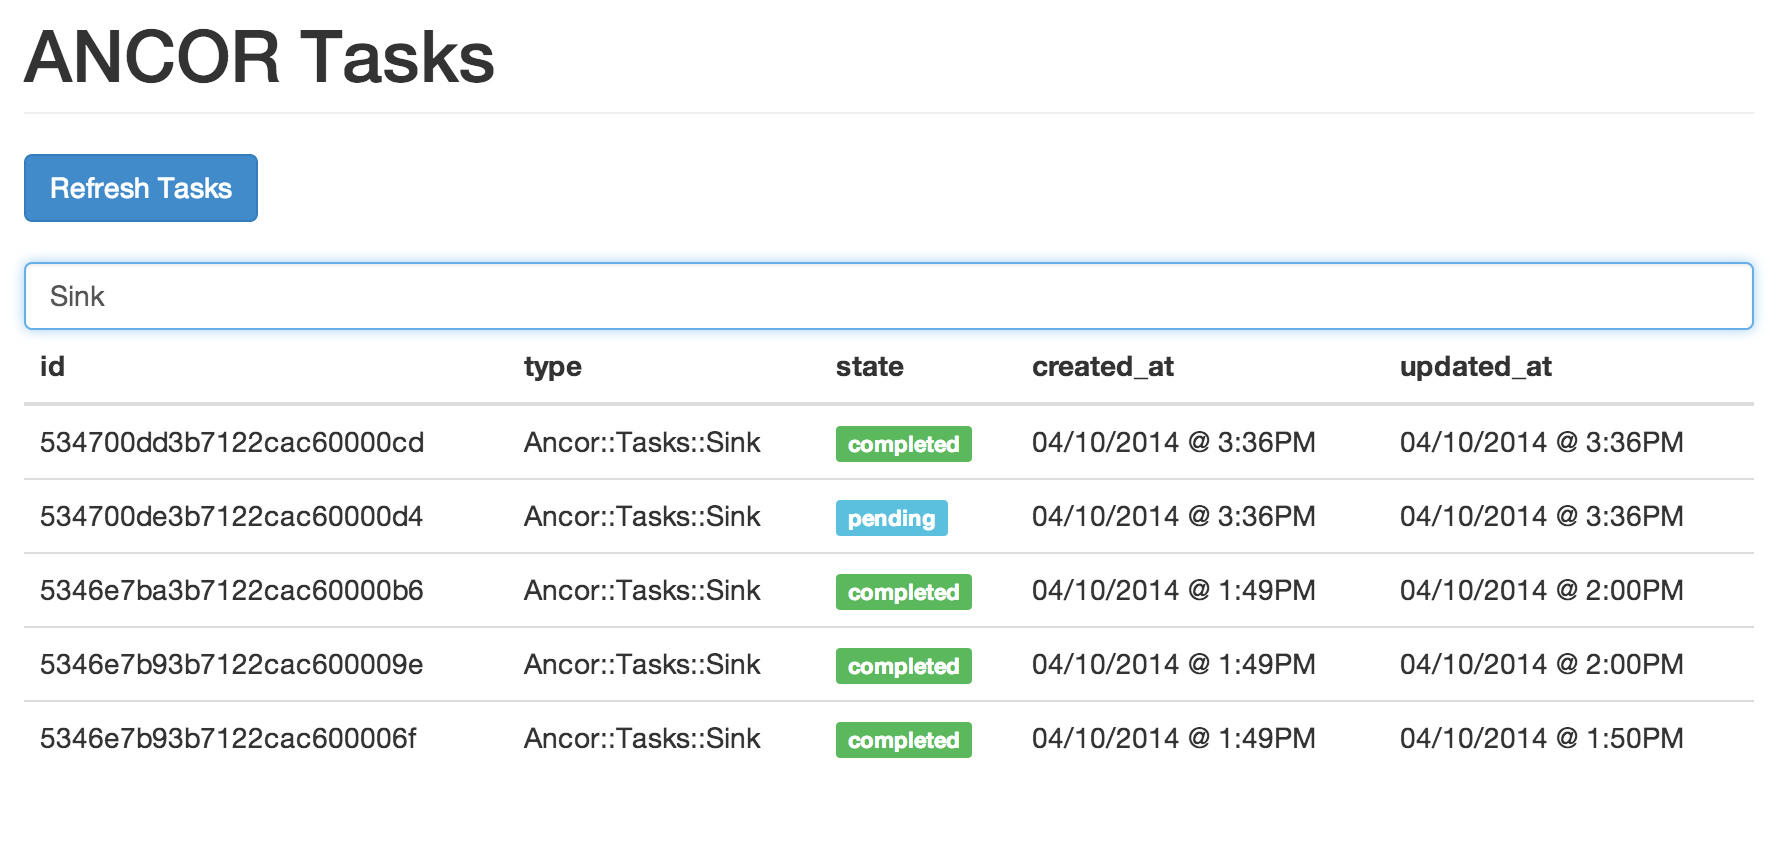
\includegraphics[height=3.0in]{figures/tasks-filter.png}

    \caption[Tasks filter view.
    ]{A filtered list of all current Tasks related to Sink.}

    \label{tasksFilter}
\end{figure}

\begin{figure}[htb]%t=top, b=bottom, h=here

    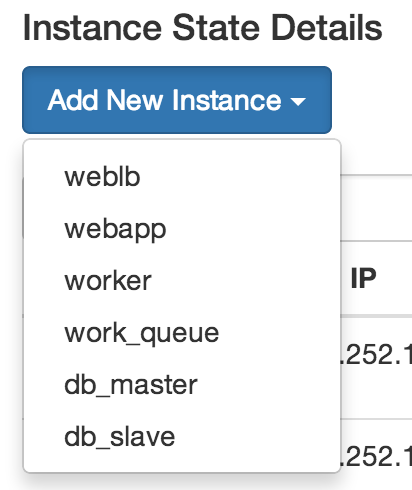
\includegraphics[height=3.0in]{figures/instance-dropdown.png}

    \caption[A dropdown of all current instances/roles.
    ]{A dropdown of all the current instances/roles to add to the deployment.}

    \label{dropdownRoles}
\end{figure}

\begin{figure}[htb]%t=top, b=bottom, h=here

    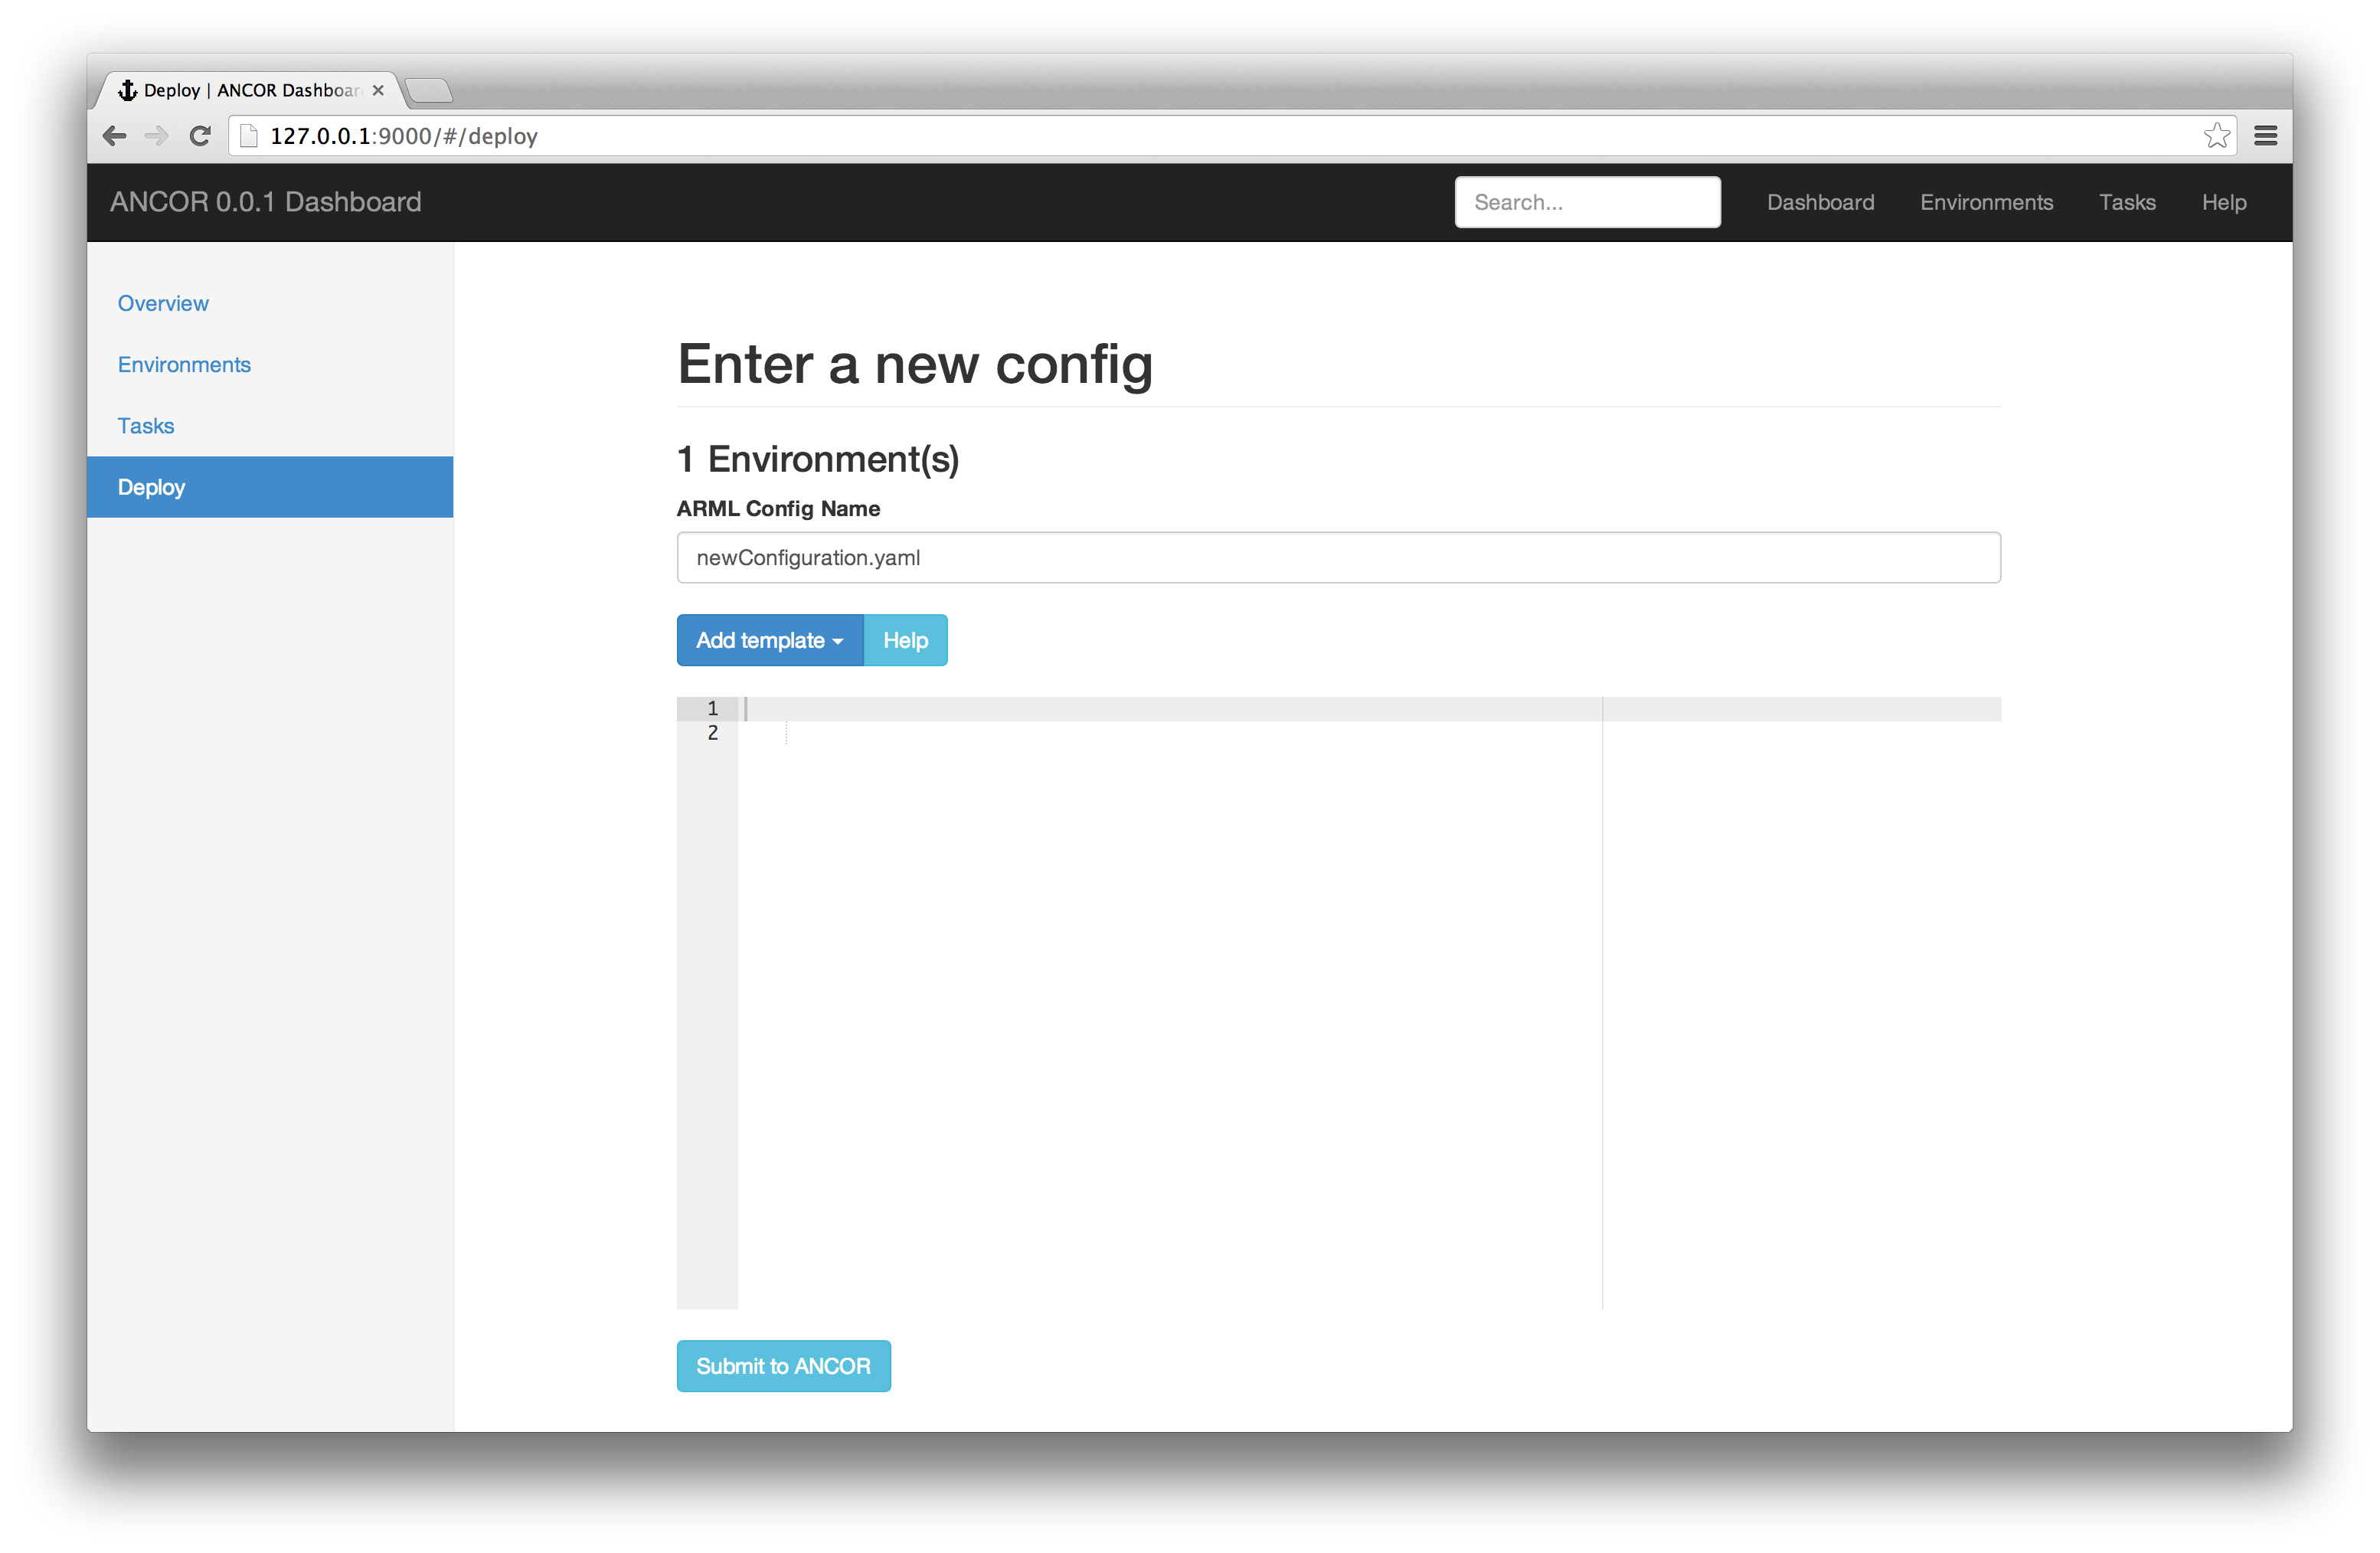
\includegraphics[height=4.0in]{figures/deploy.png}

    \caption[Deploy view.
    ]{The deploy view, where users can write their own configuration file.}

    \label{deployView}
\end{figure}

\begin{figure}[htb]%t=top, b=bottom, h=here

    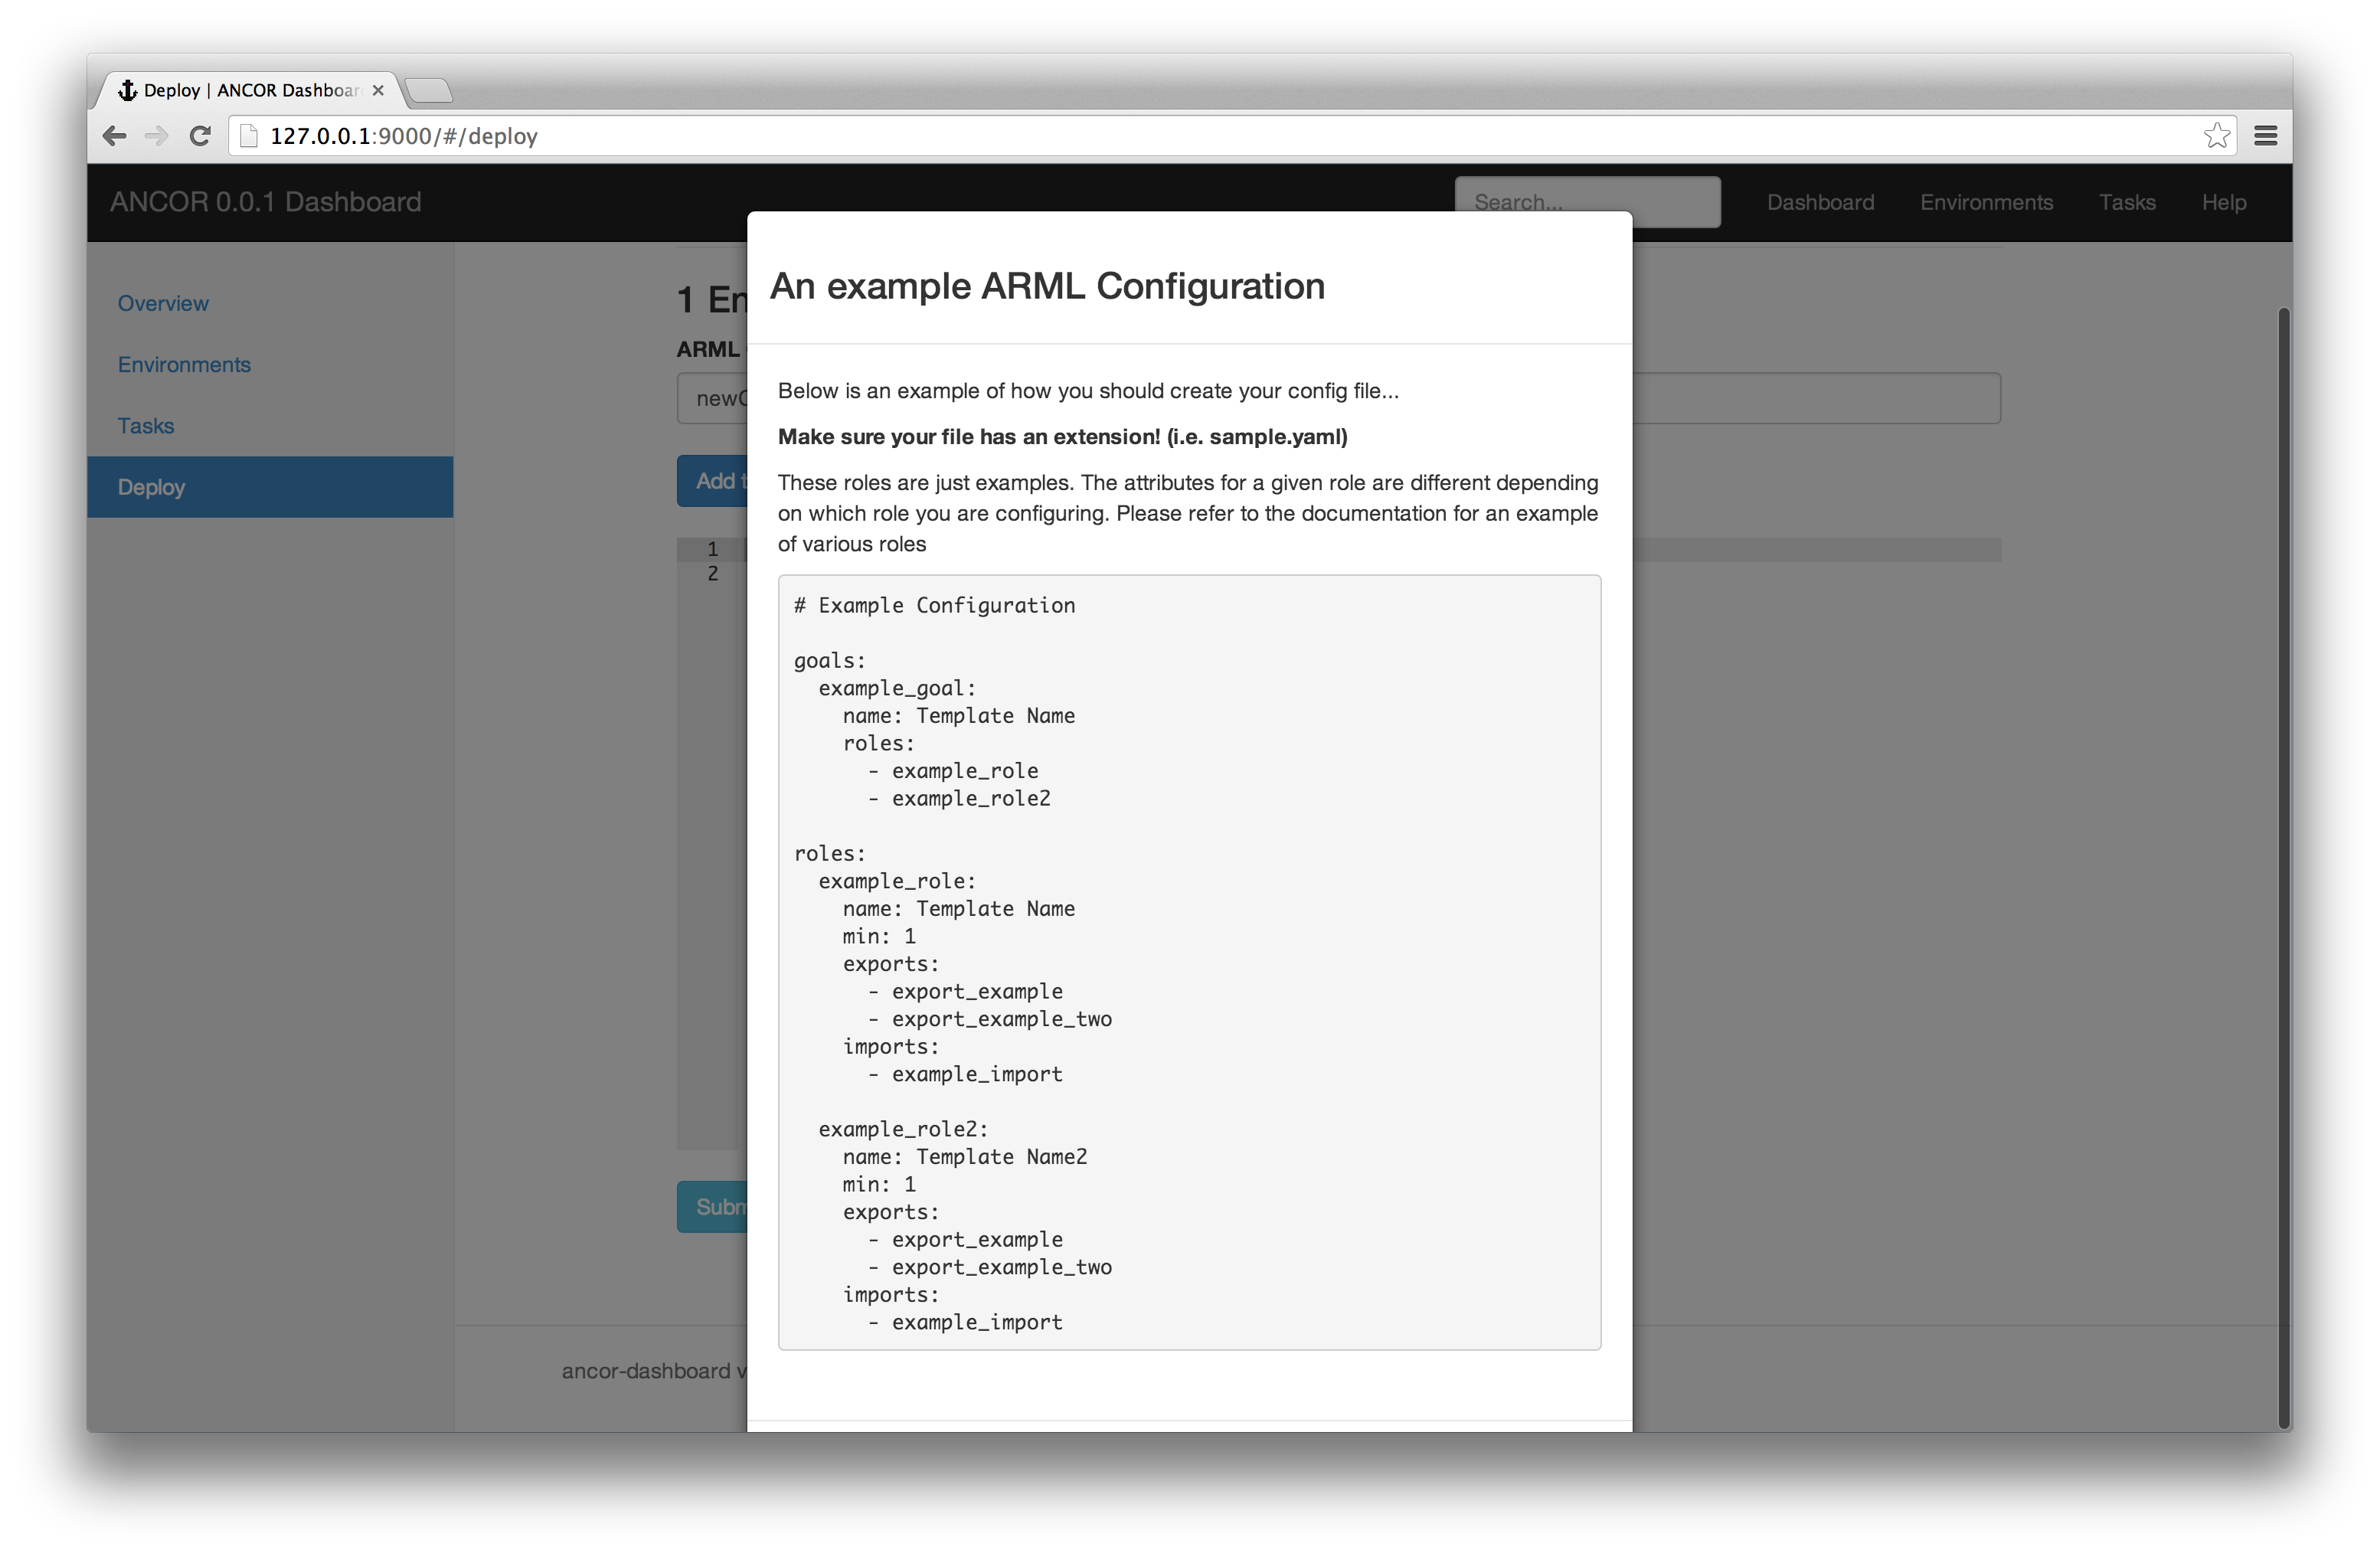
\includegraphics[height=4.0in]{figures/deploy-help.png}

    \caption[Deploy help view.
    ]{The deploy help modal view.}

    \label{deployHelpView}
\end{figure}

\begin{figure}[htb]%t=top, b=bottom, h=here

    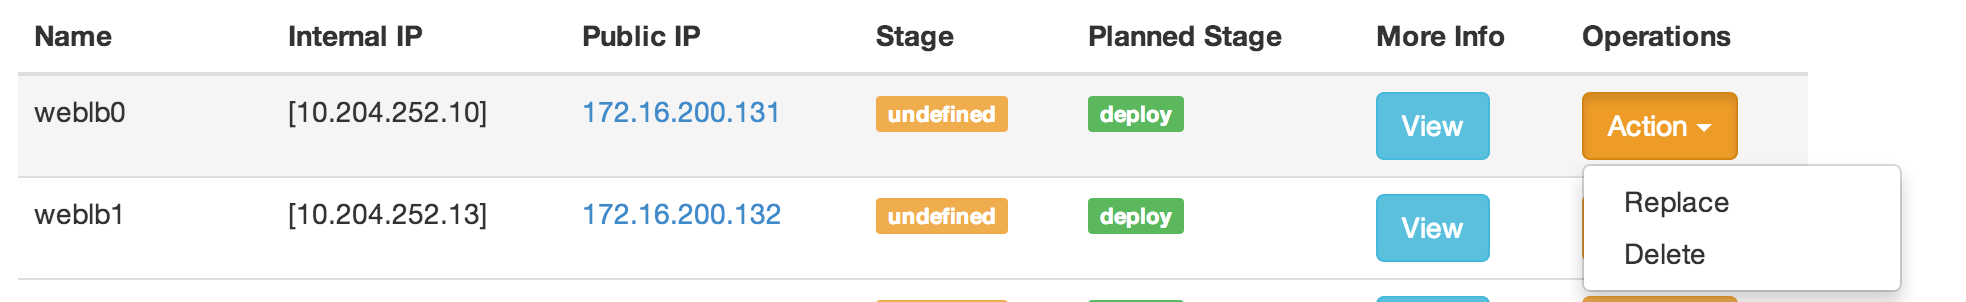
\includegraphics[height=1.0in]{figures/instance-replace-delete.png}

    \caption[Replacing or deleting an instance.
    ]{Replacing or deleting an instance.}

    \label{replaceDeleteInstance}
\end{figure}

\begin{figure}[htb]%t=top, b=bottom, h=here

    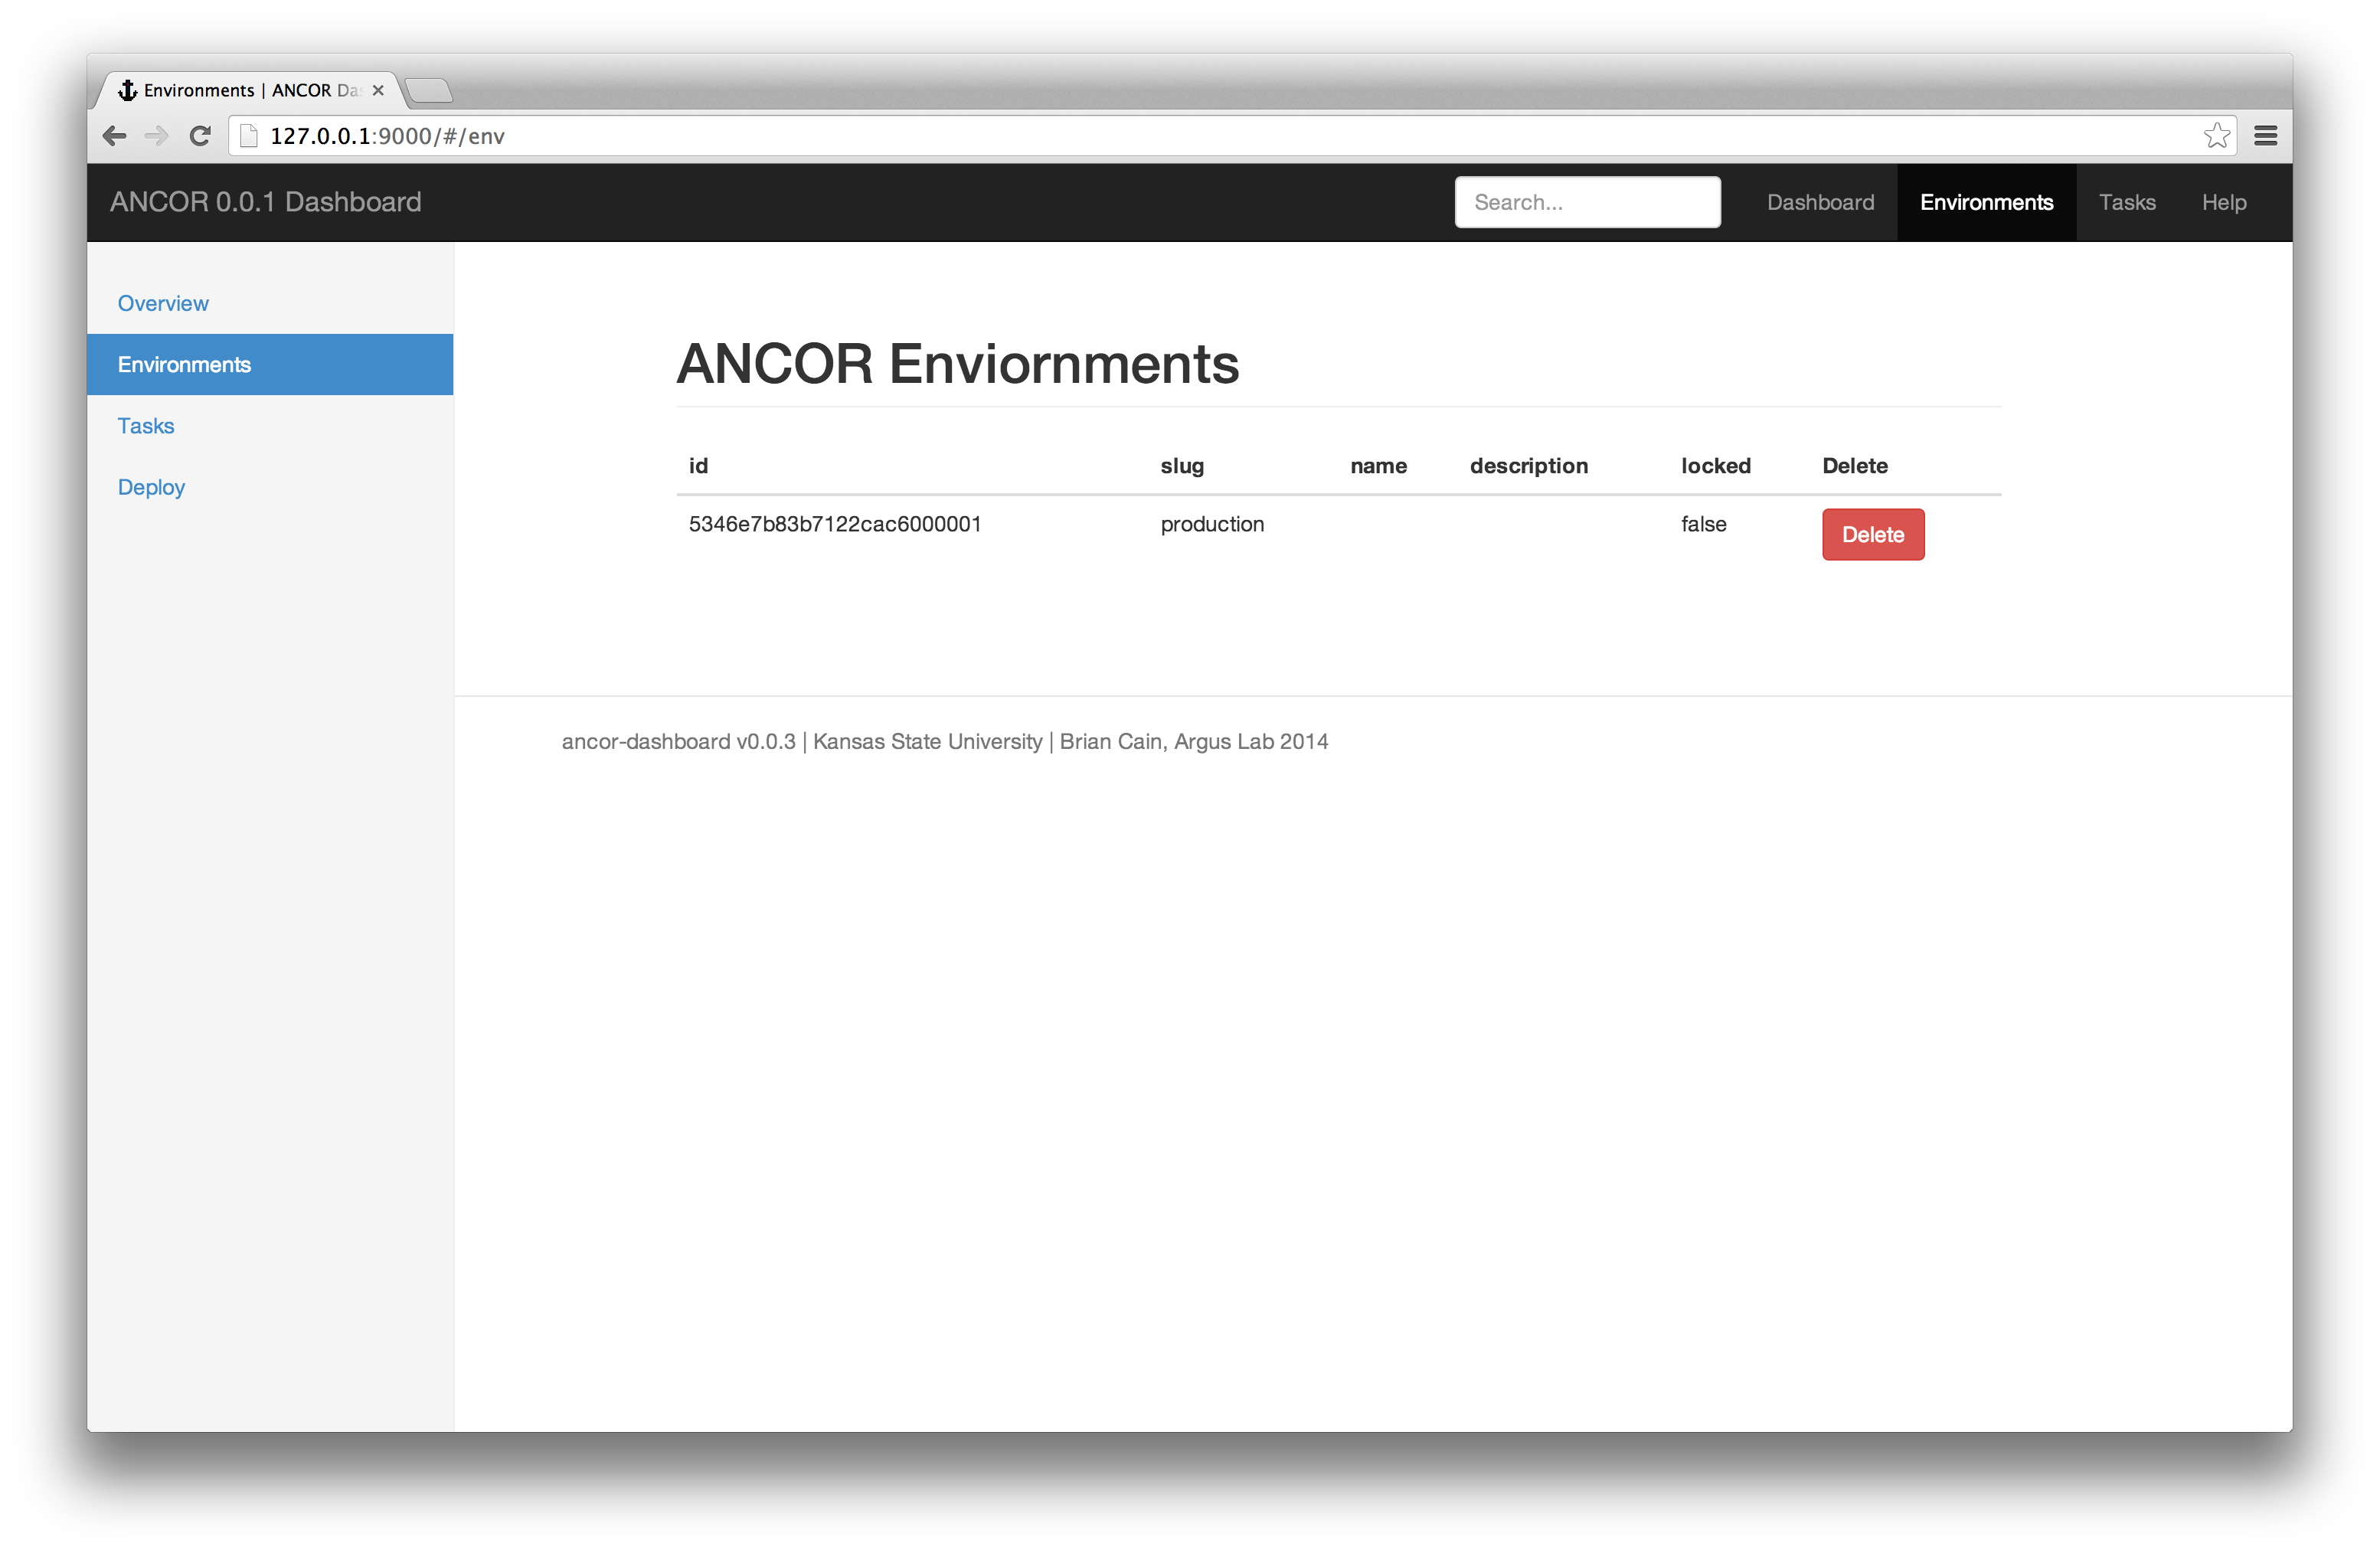
\includegraphics[height=4.0in]{figures/environments.png}

    \caption[Environments view.
    ]{The environments view.}

    \label{envView}
\end{figure}

% +--------------------------------------------------------------------+
% | Enter text for your Appendix page in the space below this box.     |
% |                                                                    |
% +--------------------------------------------------------------------+


\end{document}
